\documentclass{article}
    % General document formatting
    \usepackage[margin=0.7in]{geometry}
    \usepackage[parfill]{parskip}
    \usepackage[utf8]{inputenc}
    
    % Related to math
    \usepackage{amsmath,amssymb,amsfonts,amsthm}
\usepackage{graphicx}
%\usepackage{subfig}
%\usepackage{subfigure}
\usepackage{caption}
\usepackage{subcaption}
\usepackage{listings}

\usepackage{titling}
%\usepackage{lipsum}

\usepackage{titlesec}

\titleformat*{\section}{\Large\bfseries}
\titleformat*{\subsection}{\large\bfseries}
%\titleformat*{\subsubsection}{\large\bfseries}
%\titleformat*{\paragraph}{\large\bfseries}
%\titleformat*{\subparagraph}{\large\bfseries}
\titlespacing\section{0pt}{12pt plus 4pt minus 2pt}{0pt plus 2pt minus 2pt}
\titlespacing\subsection{0pt}{12pt plus 4pt minus 2pt}{0pt plus 2pt minus 2pt}
\titlespacing\subsubsection{0pt}{12pt plus 4pt minus 2pt}{0pt plus 2pt minus 2pt}

\pretitle{\begin{center}\large\bfseries}
\posttitle{\par\end{center}\vskip 0.01em}
\preauthor{\begin{center}\Large\ttfamily}
\postauthor{\end{center}}
\predate{\par\normalsize\centering}
\postdate{\par}

\title{Population Genetic Analyses of Genomic Data 1}
%\date{\today}


\begin{document}

%\maketitle

\begin{center}
\textbf{\Large{\centering{Computational Neruscience 1}}}\\
\textit{USN: 303039534}\\
\end{center}

%\normalsize{   }
~\\


\section{Hodgkin Huxley model}

We implement the Hodgkin Huxley model as described in Dayan and Abbott (2005), defined by equations 1-5



\begin{equation}
c_m \dfrac{dV}{dt} = -i_m + \dfrac{I_e}{A}
\end{equation}
\begin{equation}
i_m = \bar g_L(V-E_L)+ \bar g_Kn^4(V-E_K)+ \bar g_{Na}m^3h(V-E_{Na})
\end{equation}
\begin{equation}
\tau_n(V) = \dfrac{1}{\alpha_n(V) + \beta_n(V)}
\end{equation}
\begin{equation}
n_{\inf} = \alpha_n(V)\tau_n(V)
\end{equation}
\begin{equation}
\tau_n(V)\dfrac{dn}{dt}=n_{\inf}(V)-n
\end{equation}

With $\alpha_n(V)$ and $\beta_n(V)$ given in Dayan and Abbott, and including equivalent equations to (3)-(5) for gating variables $m$ and $h$.
Empirical parameters and their values taken from either the assignment description or Dayan and Abbott are given in table \ref{tab:paramshh}

\begin{table}[h]
\centering
\begin{tabular}{ |c|c|c|c|c|c|c|c|c|c|c|}
\hline
 $c_m$ &  $\bar g_L$ & $\bar g_K$ & $\bar g_{Na}$ & $E_L$ & $E_K$ & $E_{Na}$ & $V_0$ & $n_0$ & $m_0$ & $h_0$ \\
\hline
$10 \dfrac{nF}{mm^2}$ & $ 3\dfrac{\mu S}{mm^2} $ & $ 360\dfrac{\mu S}{mm^2} $& $ 1200\dfrac{\mu S}{mm^2} $& $-54.387 mV$ & $-77 mV$ & $50 mV$ & $-65 mV$ & $0.3177$ & $0.0529$ & $0.5961$ \\
\hline
\end{tabular}
\caption{Fixed parameters for Hodgkin-Huxley model}
\label{tab:paramshh}
\end{table}

The external input $I_e/A$ is varied over the course of the assignment. We integrate equations (1) and (5) using the R $deSolve$ library with a timestep of $dt=0.1$ as suggested in the assignment. Setting $I_e/A = 200 nA/mm^2$, we get spiking activity in our model neurons with a firing rate of approximately 80 hz. The model potential and gating variables are plotted for a 30ms simulation in figure 1.

\begin{figure}[h]
	\centering
	\begin{subfigure}[t]{0.45\linewidth}
		\centering
		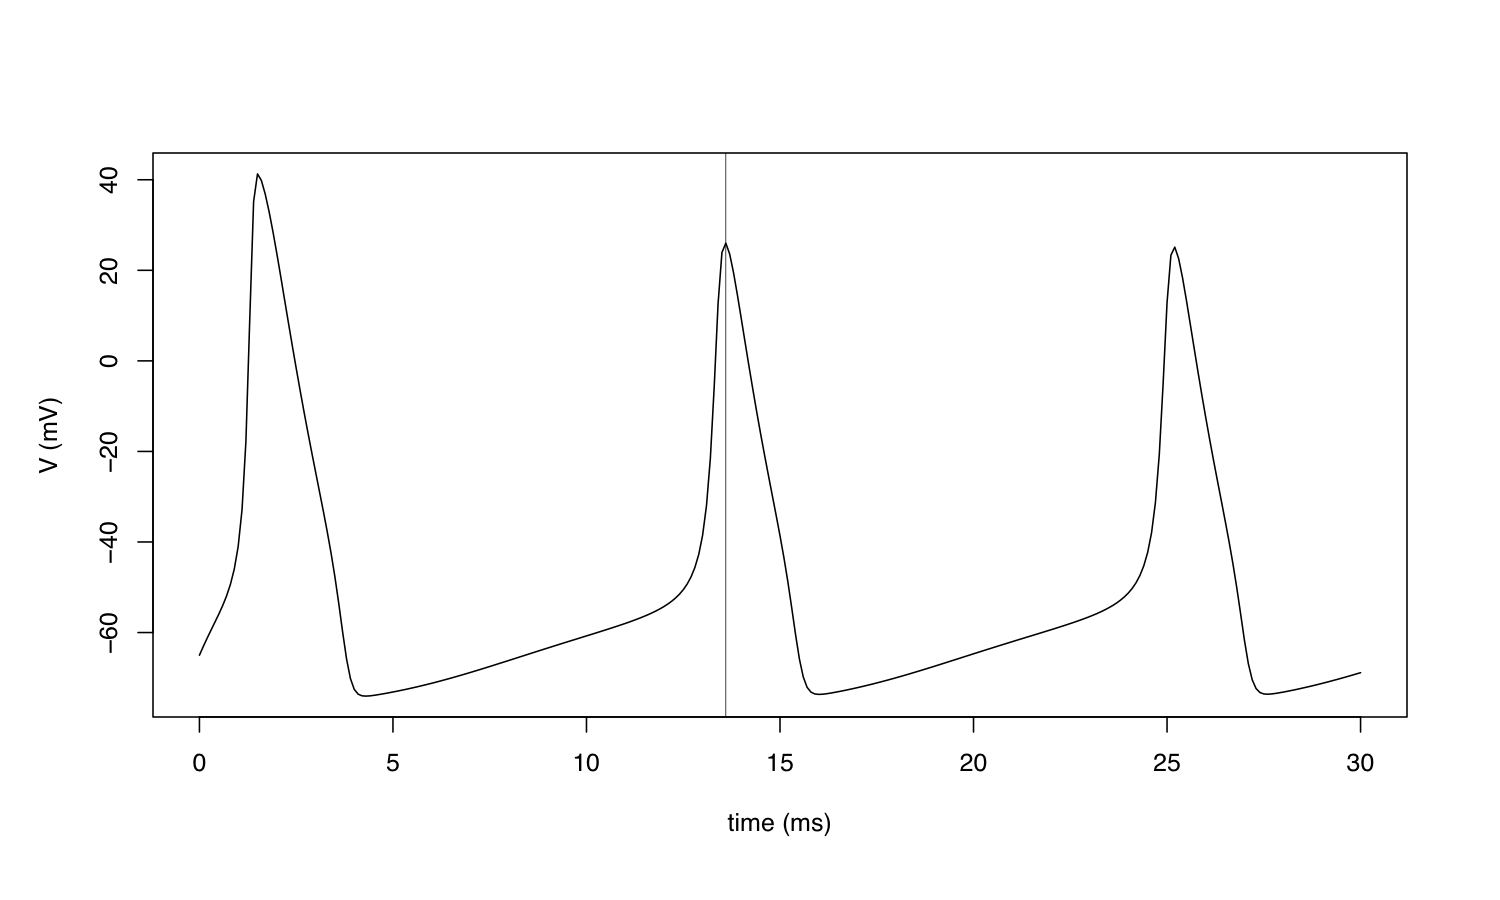
\includegraphics[width = 1.0\linewidth, trim={20 60 40 70}, clip=true]{hh_V.png}
		\subcaption{Voltage over time for a Hodking Huxley simulation}
		\label{fig:hhV}	
	\end{subfigure}%
	\hspace{0.05\linewidth}
	\begin{subfigure}[t]{0.45\linewidth}
		\centering
		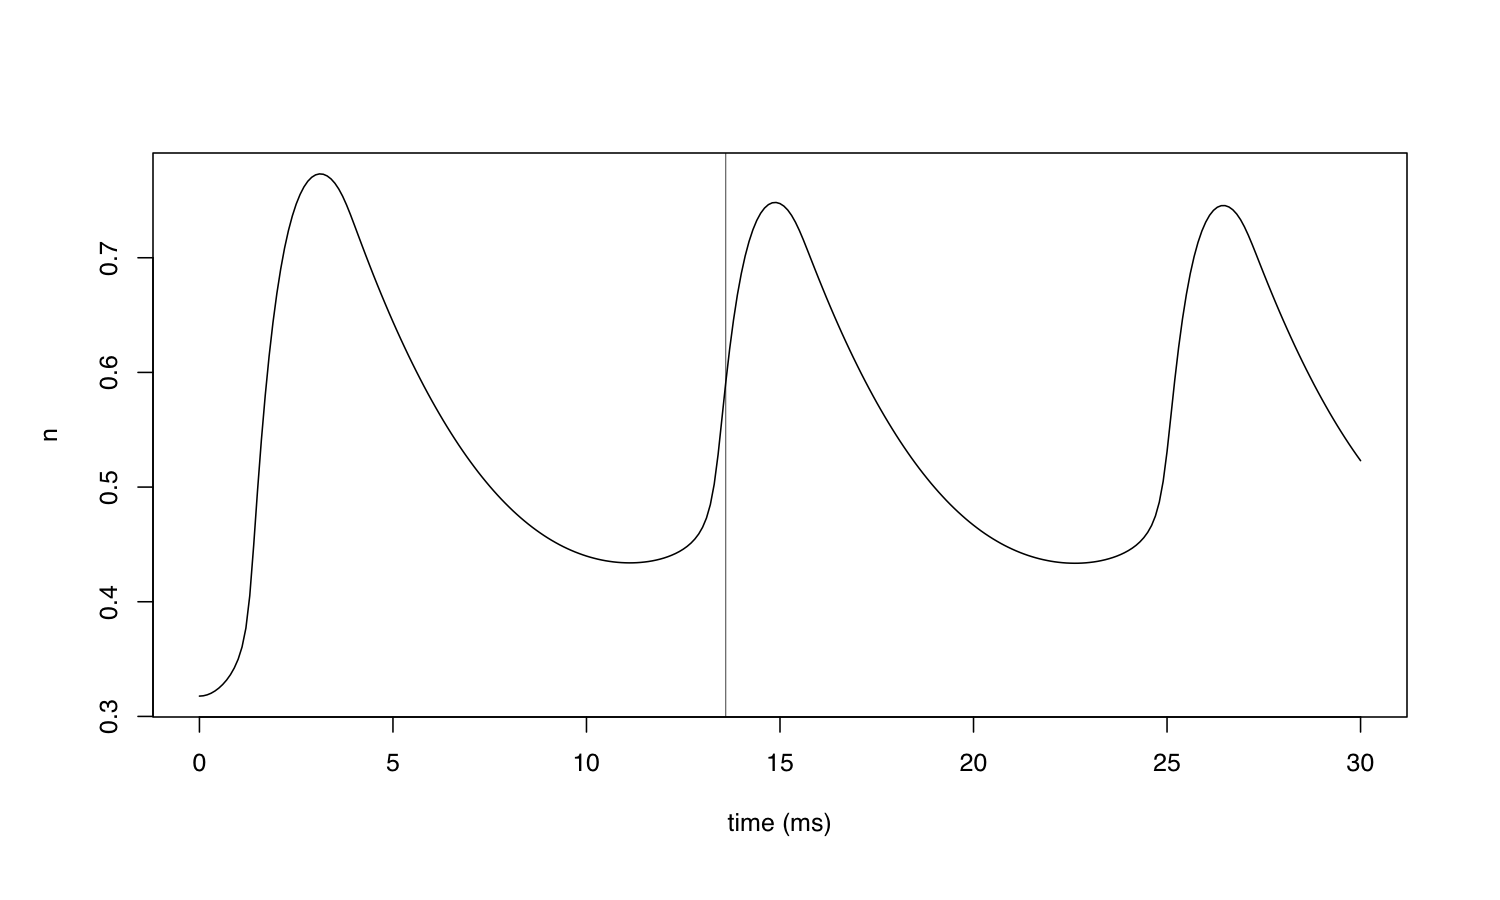
\includegraphics[width = 1.0\linewidth, trim={20 60 40 70}, clip=true]{hh_n.png}
		\subcaption{Potassium gating variable $n$}
		\label{fig:hhn}	
	\end{subfigure}%
	\hspace{0.05\linewidth}
	\begin{subfigure}[t]{0.45\linewidth}
		\centering
		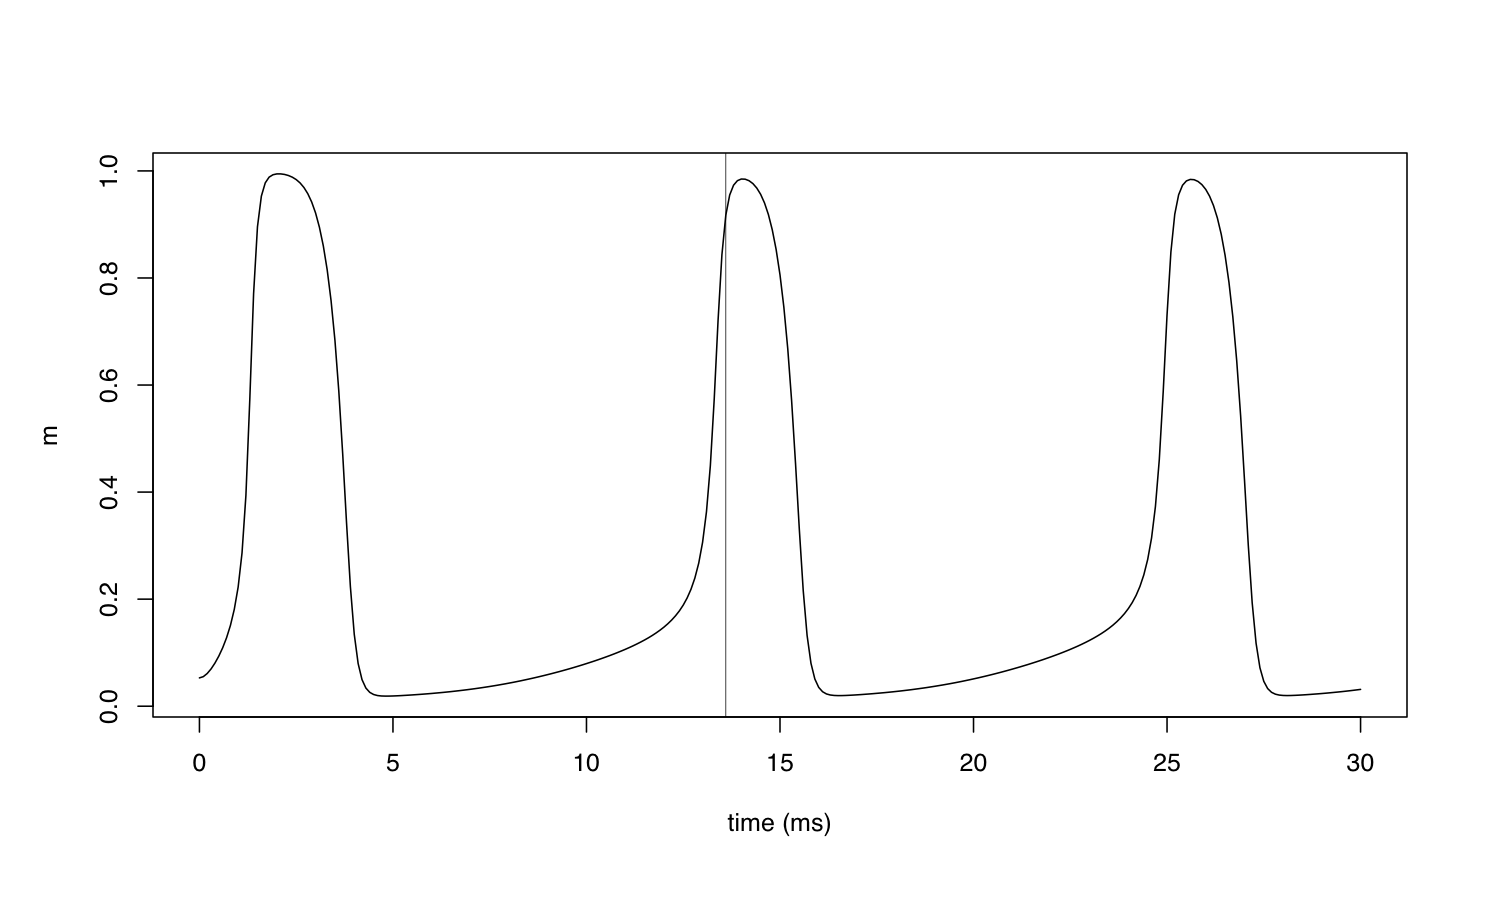
\includegraphics[width = 1.0\linewidth, trim={20 30 40 70}, clip=true]{hh_m.png}
		\subcaption{Sodium gating variable $m$}
		\label{fig:hhm}	
	\end{subfigure}%
	\hspace{0.05\linewidth}
	\begin{subfigure}[t]{0.45\linewidth}
		\centering
		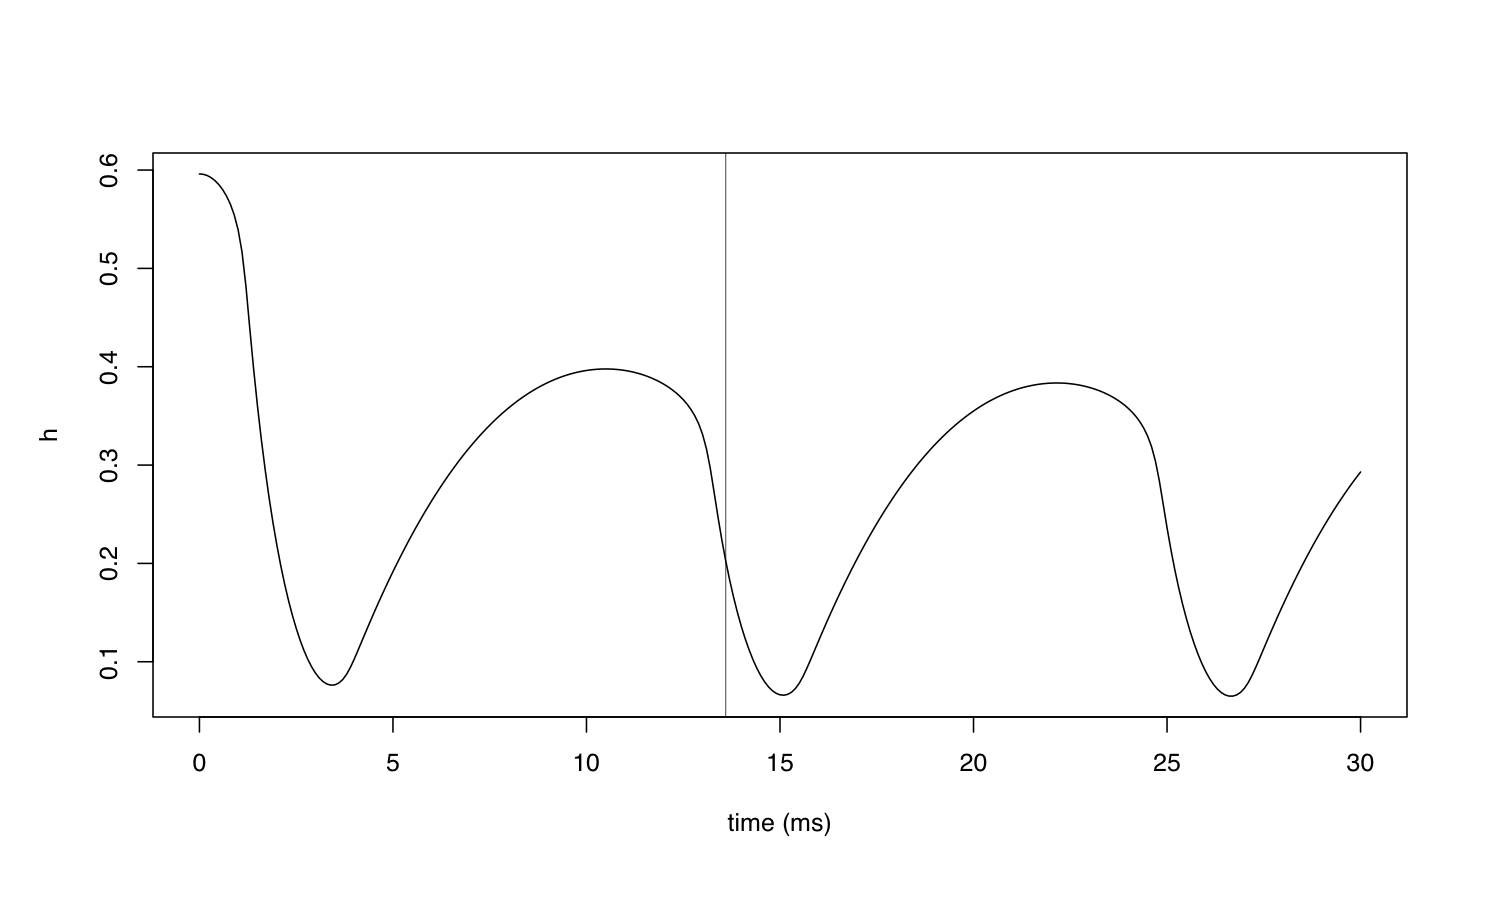
\includegraphics[width = 1.0\linewidth, trim={20 30 40 70}, clip=true]{hh_h.png}
		\subcaption{Sodium inactivation variable $h$}
		\label{fig:hhh}	
	\end{subfigure}%
%\caption{Sustained firing in a Hodgkin-Huxley model. Dashed line indicates peak of second action potential.}
\label{fig:hh}
\end{figure}

We see that as the potential increases, so does the sodium gating variable m, leading to increased sodium influx and an increase in the potential towards the sodium equilibrium potential of $E_{Na} = 50 mV$. However, this also drives the sodium inactivation variable h to 0 with a longer time constant, which terminates the sodium influx. In combination with an increase in the value of the potassium gating variable m, this leads to a decrease in the potential as it approaches the potassium equilibrium potential of $E_K = -77 mV$.

In figure 1 the apiking activity is driven by the external input $I_E/A$, and we can investigate the effect of this variable on the behavior of the system (\ref{fig:rates}). If we denote the time difference between the two final spikes of our system as $\Delta T$, we define the equilibrium firing rate as $\omega = \dfrac{1}{\Delta T}$ and require the final spike to occur within $\Delta T$ of terminating the simulation to ensure sustained firing.
In this case we do not need to average over multiple spikes since the simulation is deterministic with no stochastic component. We define a spike as a local maximum in V with V>0.

\begin{figure}[h]
\begin{subfigure}[t]{0.48\linewidth}
	\centering
	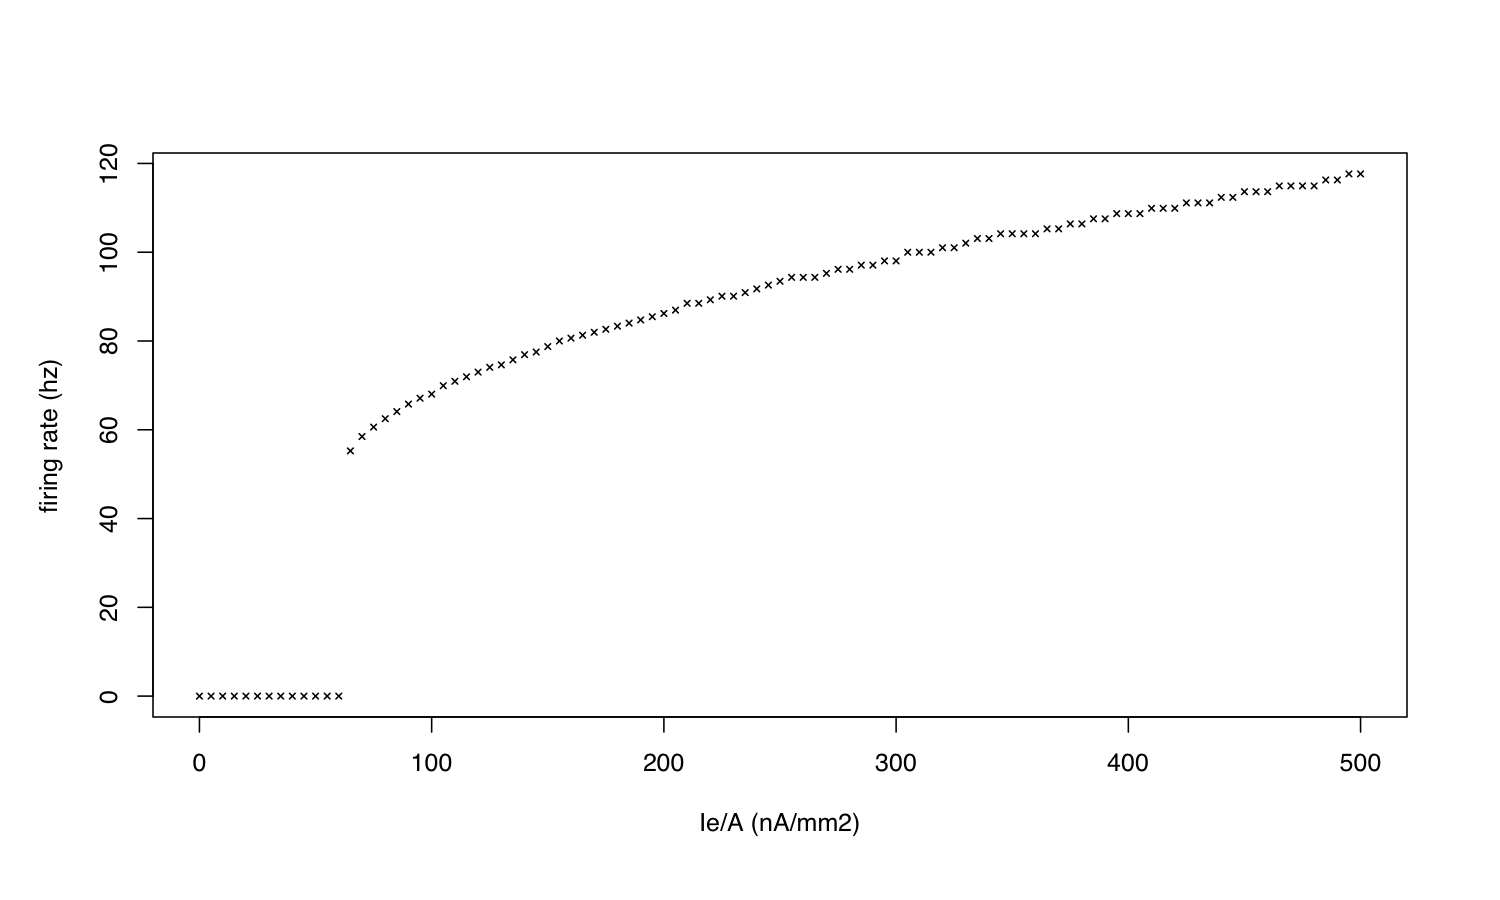
\includegraphics[width = 1.0\linewidth, trim={20 30 40 70}, clip=true]{firing_rates.png}
	\label{fig:bigrates}	
\end{subfigure}
\hspace{0.02\linewidth}
\begin{subfigure}[t]{0.48\linewidth}
	\centering
	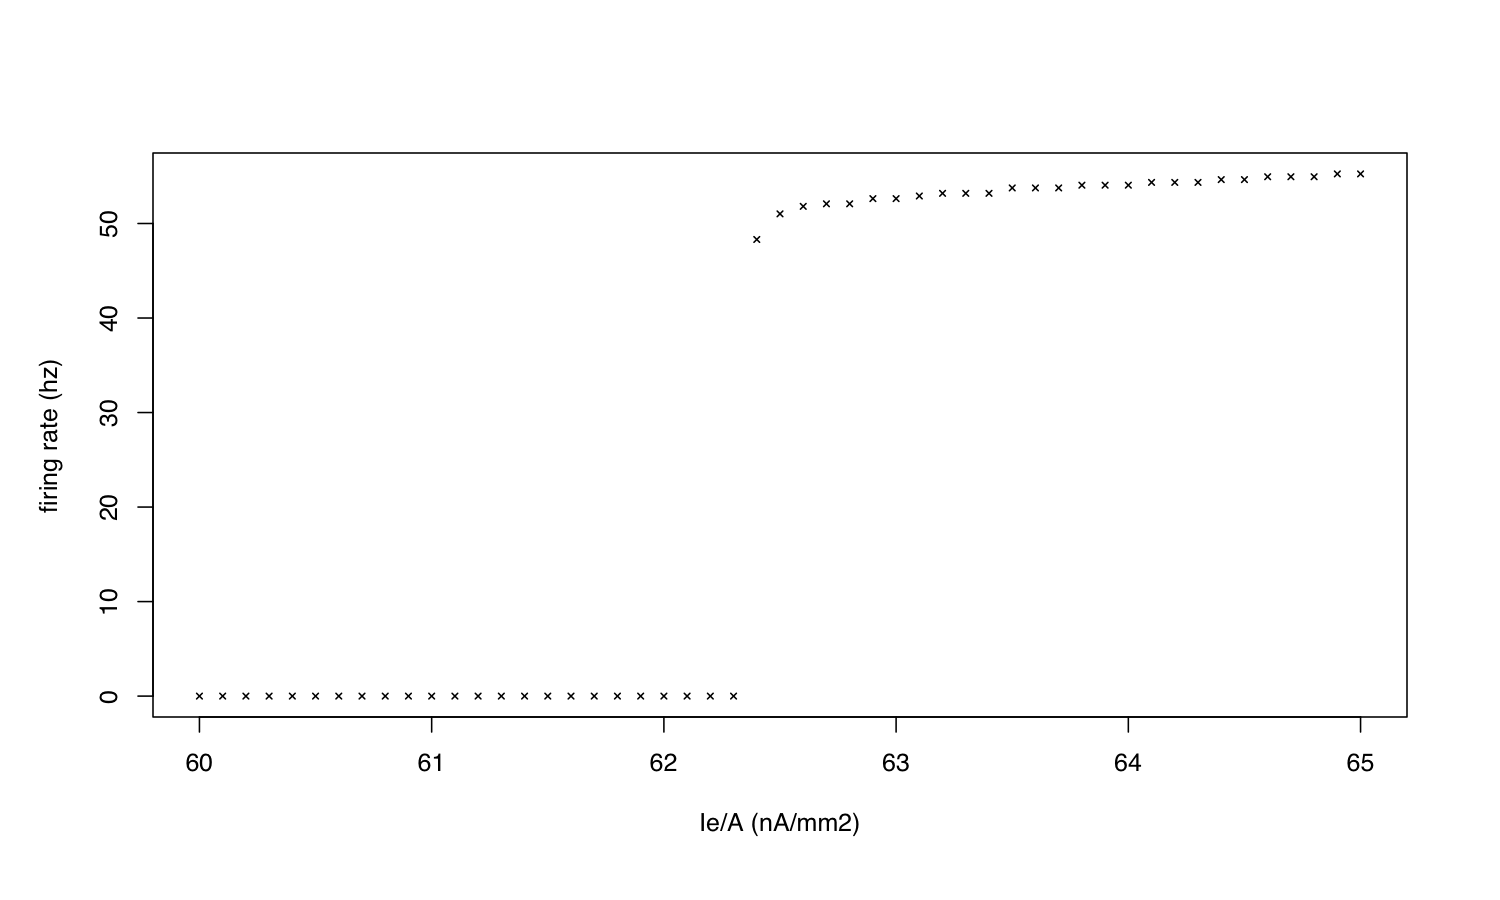
\includegraphics[width = 1.0\linewidth, trim={20 30 40 70}, clip=true]{firing_rates_finegrained.png}
	\label{fig:smallrates}	
\end{subfigure}
\label{fig:rates}
\caption{Sustained firing rate as a function of external input. \textit{left:} scanning the range $I_e/A \in [0:500]$, we find a firing rate of zero at low input and a firing rate linear in $I_e/A$ at high input. \textit{right:} zooming in on the region $I_e/A \in [60:65]$ we find a discontinous jump in the firing rate from 0 to 50 between $62.3$ and $62.4 nA/mm^2$. }
\end{figure}

We see from figure \ref{fig:rates}a that for high external inputs, the firing rate is approximately linear in $I_e/A$. For small external input, the leak from the neuron is sufficient to prevent the potential from reaching threshold and we thus see a firing rate of 0. We find that there is a switch between these two behaviors between $I_e/A = 60$ and $I_e/A = 65$ and expand this region in figure \ref{fig:smallrates}b. Even at this high resolution, we find the transition to be discontinuous; if $I_e/A < 62.35$ there is no firing and the neuron is at steady state, while if $I_e/A > 62.35$ the system exceeds threshold and we get a finite firing rate of 50 hz.

Finally we consider what happens in the case of an inhibitory external input with $I_e/A = -50 nA/mm^2$ for 5 ms followed by removing all external input. The current and gating variables for such a system are plotted in figure \ref{fig:hh_jump}. 


\begin{figure}[h]
	\centering
	\begin{subfigure}[t]{0.45\linewidth}
		\centering
		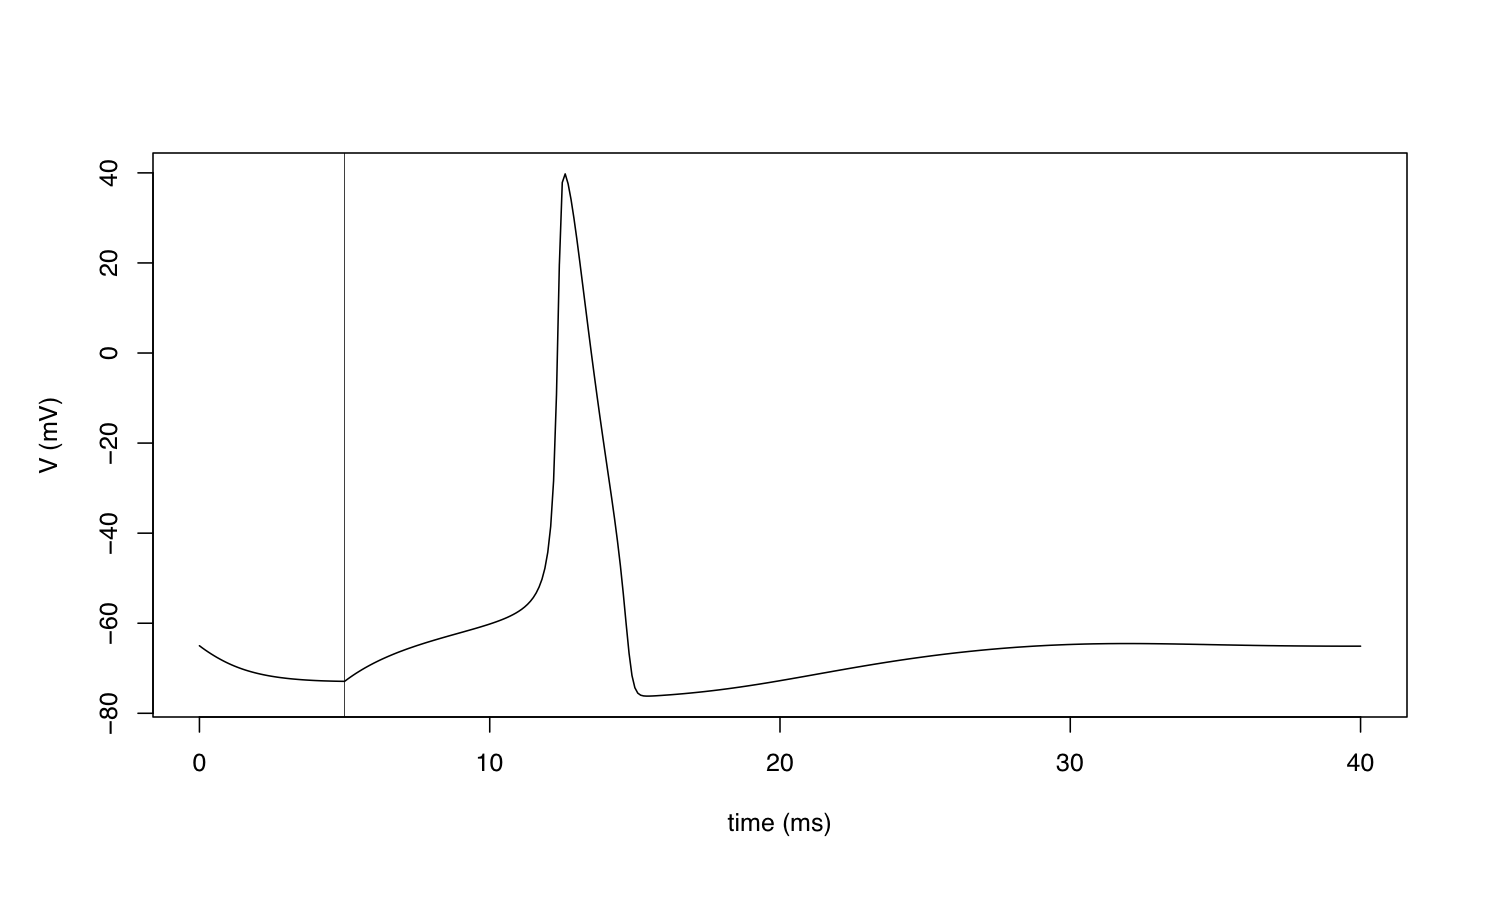
\includegraphics[width = 1.0\linewidth, trim={20 60 40 70}, clip=true]{hh_jump_V.png}
		%\subcaption{Voltage over time for Vinit = -60, -80}
		\label{fig:hhV}	
	\end{subfigure}%
	\hspace{0.05\linewidth}
	\begin{subfigure}[t]{0.45\linewidth}
		\centering
		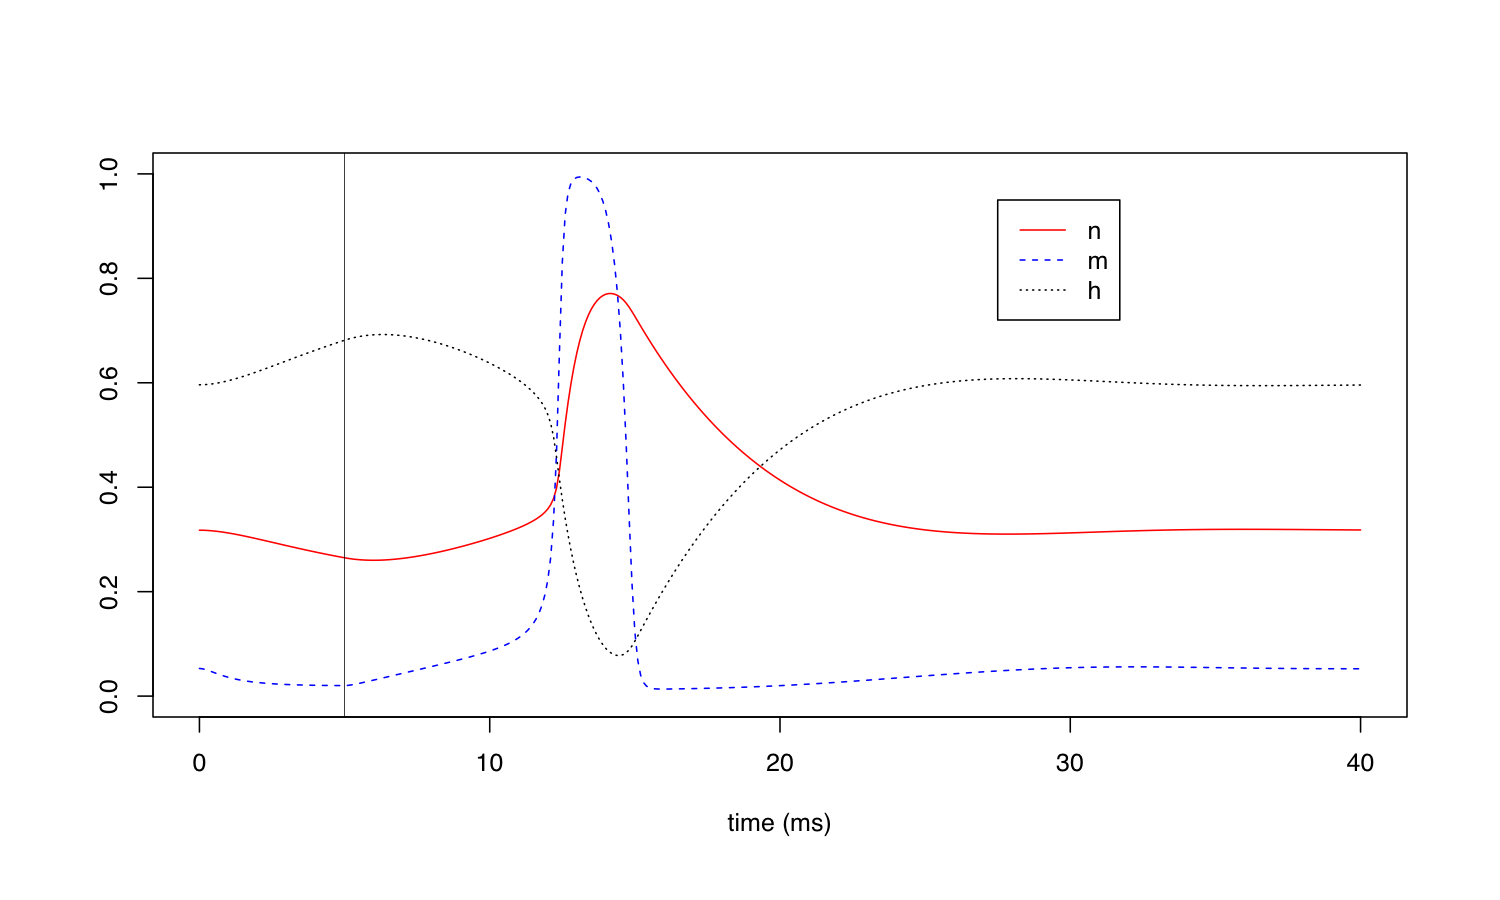
\includegraphics[width = 1.0\linewidth, trim={20 60 40 70}, clip=true]{hh_jump_gating.png}
		%\subcaption{Voltage over time for Vinit = -60, -80}
		\label{fig:hhV}	
	\end{subfigure}%

\caption{Hodgkin-Huxley model showing a post-inhibitory rebound following brief repression. (\textit{left}) potential as a function of time. (\textit{right}) gating variables $n, m$ \& $h$. Dashed line indicates $t=5ms$ when repression is relieved.}
\label{fig:hh_jump}
\end{figure}

Surprisingly, we find that the neuron fires exactly once after the removal of the external input, following which it returns to steady state. We can understand this behavoir by looking at what happens to the gating variables. At $t=5ms$ following inhibition, $m$ has been driven to near $0$ while $h=0.68$. This mean that upon relief of inhibition, conditions are such that there is a rapid influx of sodium at a shorter timescale than $\tau_n = 5.75$ and $\tau_h=7.93$ under these conditions. The neuron therefore reaches threshold and fires a spike. However, after the refractory period there is no input to drive the neuron to threshold again, and it reaches an equilibrium state of $-65 mV$ where $i_m$ = 0.

\section{Coupled integrate and fire neurons}

We implement a set of two coupled integrate and fire neurons. These evolve over time according to

\begin{equation}
\tau_m \dfrac{dV}{dt} = E_L - V - r_m \bar g_s P_s(V-E_S) + R_m I_e
\end{equation}
Here, $r_m$ is the membrane resistance, $\bar g_s$ is the synaptic conductance when the synapse is active, $P_s$ is the probability of the synapse being open, and $R_mI_e$ is the external input.

We further model $P_s$ according to equations

\begin{equation}
\tau_s \dfrac{dP}{dt} = \exp{[1]}P_{max}z-Ps
\end{equation}
\begin{equation}
\tau_s \dfrac{dz}{dt} = -z
\end{equation}

Here $z_i$ is a synaptic gating variable that is set to 1 whenever neuron $j$ fires. We set dt to 0.005 since decreasing dt further does not affect spike times in the case of either excitatory or inhibitory connections. We further use parameters in table \ref{tab:paramsif} unless otherwise stated.

\begin{table}[h]
\centering
\begin{tabular}{ |c|c|c|c|c|c|c|c|c|c|}
\hline
 $E_L$ &  $V_{th}$ & $V_{reset}$ & $\tau_m$ & $r_m \bar g_s$ & $R_m I_e$ & $\tau_s$ & $P_{max}$ & $E_{S; excitatory}$ & $E_{S, inhibitory}$\\
\hline
$-70 mV $ & $ -54 mV $ & $ -80 mV $ & $ 20 ms $ & $ 0.15 $ & $18 mV$ & $10 ms$ & $0.5$ & $0 mV$ & $-80 mV$\\
\hline
\end{tabular}
\caption{Parameters for integrate and fire model}
\label{tab:paramsif}
\end{table}

To investigate this system in a simple setting, we connect the two neurons via excitatory synapses and plot the voltage of each neuron as a function of time (figure \ref{fig:IFe}).

\begin{figure}[h]
	\centering
	\begin{subfigure}[t]{0.30\linewidth}
		\centering
		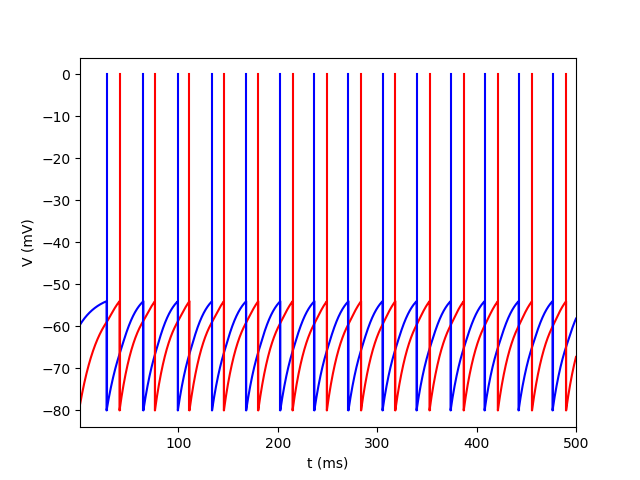
\includegraphics[width = 1.0\linewidth, trim={0 0 0 0}, clip=true]{V_60_80e.png}
		\subcaption{Voltage of two excitatory for the first 500 ms of a simulation with $V_{init} = (-60, -80)$}
		\label{fig:V80e}	
	\end{subfigure}%
	\hspace{0.03\linewidth}
	\begin{subfigure}[t]{0.30\linewidth}
		\centering
		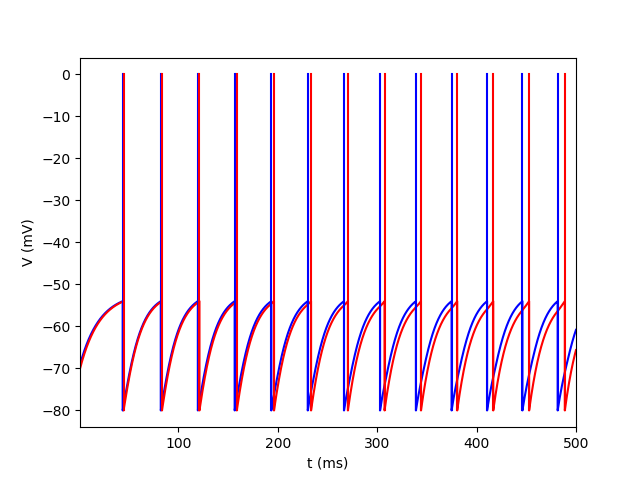
\includegraphics[width = 1.0\linewidth, trim={0 0 0 0}, clip=true]{V_70_71e.png}
		\subcaption{Voltage of two excitatory for the first 500 ms of a simulation with $V_{init} = (-71, -72)$}
		\label{fig:V71e}	
	\end{subfigure}%
	\hspace{0.03\linewidth}
	\begin{subfigure}[t]{0.30\linewidth}
		\centering
		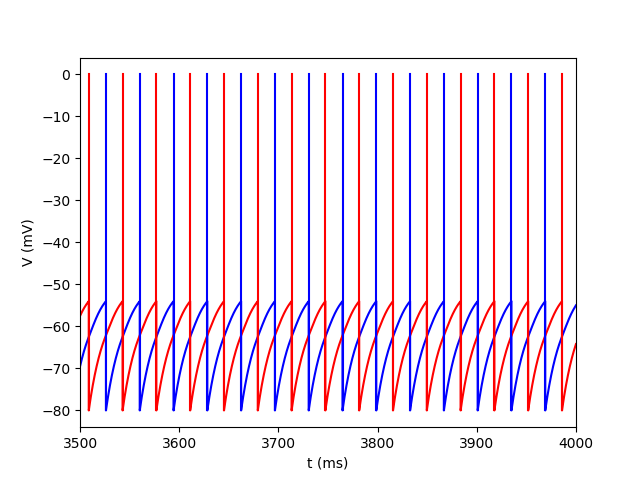
\includegraphics[width = 1.0\linewidth, trim={0 0 0 0}, clip=true]{V_70_71e_late.png}
		\subcaption{Voltage of two excitatory for 500 ms after 3500 ms of a simulation with $V_{init} = (-71, -72)$}
		\label{fig:V71e_late}	
	\end{subfigure}%
\caption{Excitatory neurons}
\label{fig:IFe}
\end{figure}

We see that in the case of excitatory neurons with default parameters, it appears that large differences in initial conditions initially lead to alternate firing while very similar initial conditions lead to near-synchronous firing. However, if we let the simulation run until threshold is reached at $t=3500$ when interspike intervals become constant, we find that the simulation with $V_{init} = (-71, -72)$ also exhibits alternate firing.
It thus appears that the equilibrium state of the system depends on the hyperparameters in table \ref{tab:paramsif} but not on the initial conditions.

To investigate the effects of initial conditions, the synaptic time constant $\tau_s$ and the synaptic strength $\rm \bar gs$ further, we quantify the interspike interval as a function of time for different conditions. Here, the interspike interval is defined as the phase difference between neuron 1 and neuron 2 and quantified by looking at the difference in time to the nearest spike of neuron 2 for a given spike in neuron 1.

We see in figure \ref{fig:intse} that for the default parameters, the initial potentials affect the interspike interval at early times, but that this difference eventually disappears since all the simulations approach an interspike interval of 16 ms corresponding to alternate firing.

The same pattern is observed when increasing $\tau_s$ from 10ms to 20ms where differences in interspike interval also decrease over time. However, in this case the interspike intervals converge more slowly as would be expected from slower coupling between the neurons. We find that they also converge to a lower interspike interval due to a higher equilibrium firing rate. This is at first surprising given the increased time constant, but on a second thought reasonable as the larger time constant broadens the synaptic current curve and leads to higher total current flow between the two neurons over the course of a synaptic event.


\begin{figure}[h]
	\centering
	\begin{subfigure}[t]{0.30\linewidth}
		\centering
		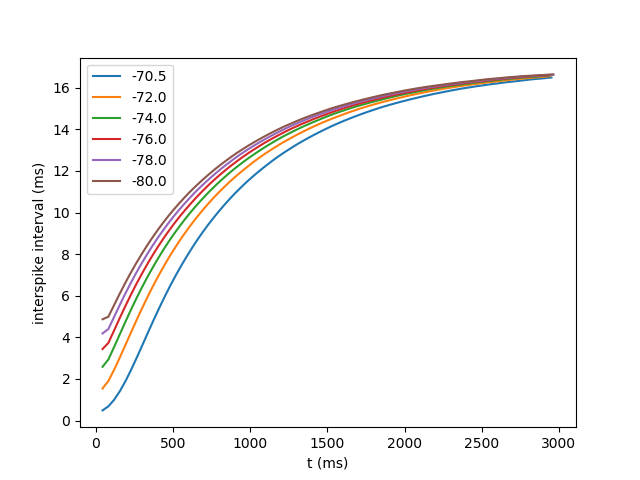
\includegraphics[width = 1.0\linewidth, trim={20 10 20 20}, clip=true]{intervals_ts_10_rmgs_015e.png}
		\subcaption{$\tau_s = 10$}
		\label{fig:ts10e}	
	\end{subfigure}%
	\hspace{0.03\linewidth}
	\begin{subfigure}[t]{0.30\linewidth}
		\centering
		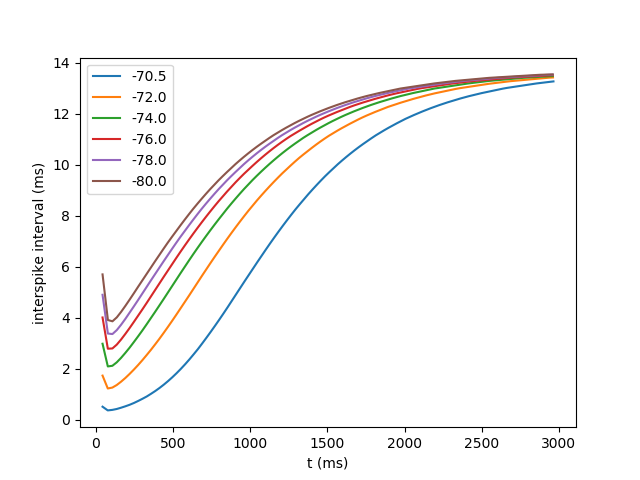
\includegraphics[width = 1.0\linewidth, trim={20 10 20 20}, clip=true]{intervals_ts_20_rmgs_015e.png}
		\subcaption{$\tau_s = 20$}
		\label{fig:ts20e}	
	\end{subfigure}%
	\hspace{0.03\linewidth}
	\begin{subfigure}[t]{0.30\linewidth}
		\centering
		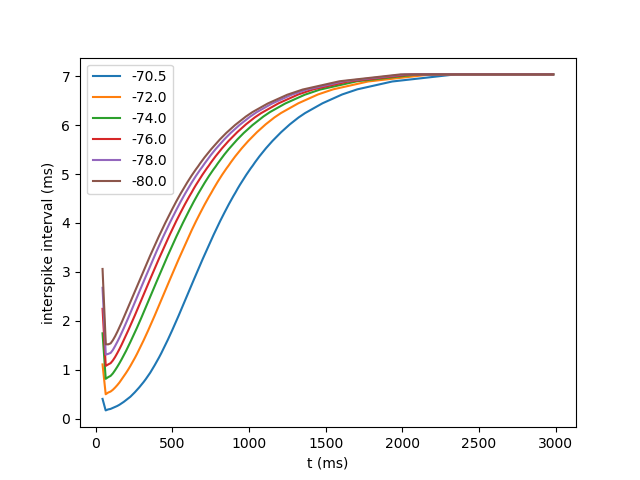
\includegraphics[width = 1.0\linewidth, trim={20 10 20 20}, clip=true]{intervals_ts_10_rmgs_05e.png}
		\subcaption{$\tau_s = 10$ $rmgs = 0.5$}
		\label{fig:ts10rmgs}	
	\end{subfigure}%
\caption{Interspike interval over time for a pair of excitatory neurons with different physical parameters. In every case, neuron 1 was initialized at $-70 mV$ and each line corresponds to a different $V_init$ of neuron 2, ranging from $-70.5$ to $-80$.}
\label{fig:intse}
\end{figure}

When increasing the synaptic strength from figure \ref{fig:ts10e} to figure \ref{fig:ts10rmgs} we also observe an increased firing rate as is expected from increasing the current flow between two excitatory neurons. The neurons with a higher synaptic strength also converge to alternate firing quicker than in figure \ref{fig:ts10e} .

We can perform similar analyses for inhibitory neurons, with equivalent plots to figures \ref{fig:IFe} and \ref{fig:intse} given in figures \ref{fig:IFi} and \ref{fig:intsi}. In contrast to the excitatory neurons, we find the long-term behavior of a system of inhibitory neurons to depend strongly on the initial state of the system.


\begin{figure}[h]
	\centering
	\begin{subfigure}[t]{0.45\linewidth}
		\centering
		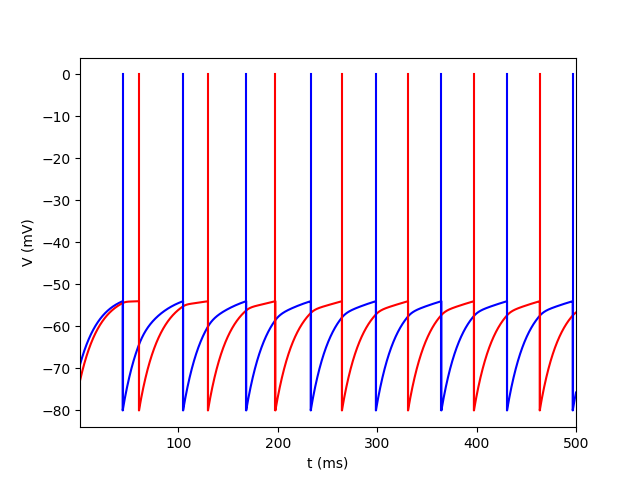
\includegraphics[width = 1.0\linewidth, trim={0 0 0 0}, clip=true]{V_74i.png}
		\subcaption{Voltage over time for Vinit = -70, -74}
		\label{fig:V74}	
	\end{subfigure}%
	\hspace{0.05\linewidth}
	\begin{subfigure}[t]{0.45\linewidth}
		\centering
		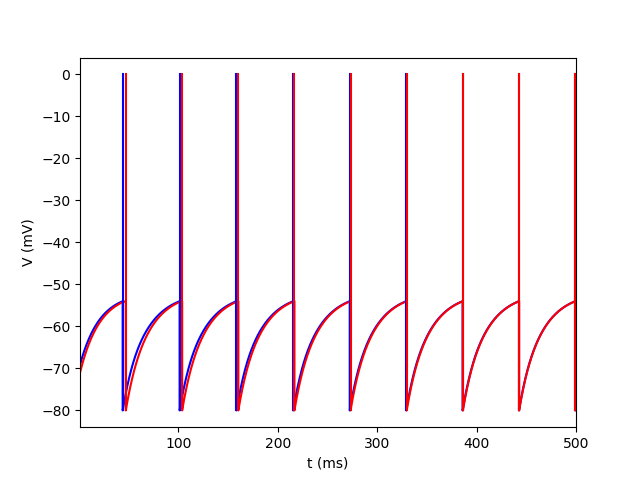
\includegraphics[width = 1.0\linewidth, trim={0 0 0 0}, clip=true]{V_72i.png}
		\subcaption{Voltage over time for Vinit = -70, -72}
		\label{fig:V72}	
	\end{subfigure}%
\caption{Inhibitory neurons}
\label{fig:IFi}
\end{figure}

\begin{figure}[h]
	\centering
	\begin{subfigure}[t]{0.30\linewidth}
		\centering
		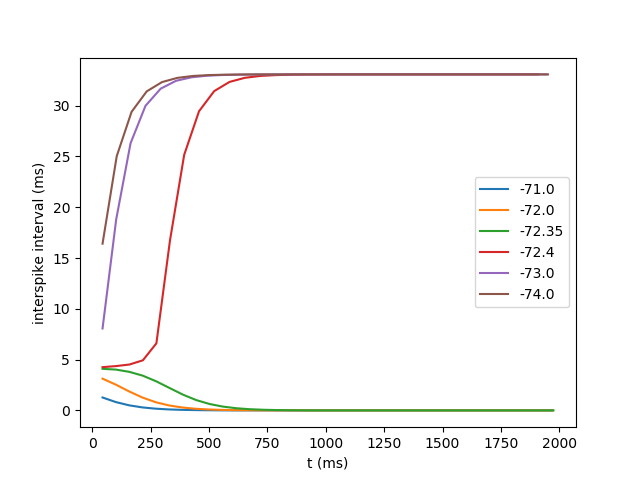
\includegraphics[width = 1.0\linewidth, trim={20 10 20 20}, clip=true]{intervals_ts_10i.png}
		\subcaption{$\tau_s = 10$}
		\label{fig:ts10}	
	\end{subfigure}%
	\hspace{0.03\linewidth}
	\begin{subfigure}[t]{0.30\linewidth}
		\centering
		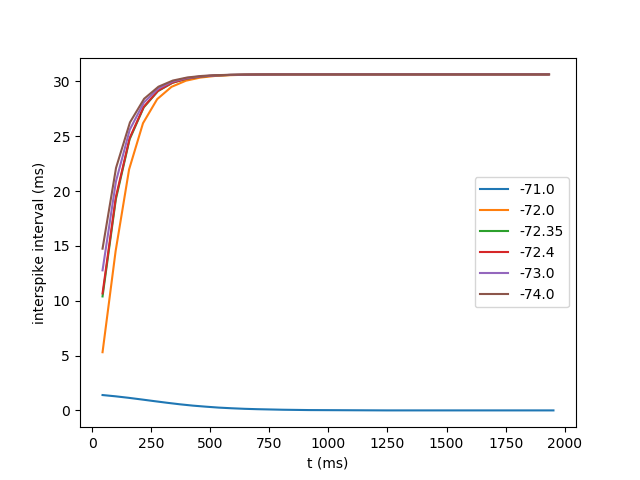
\includegraphics[width = 1.0\linewidth, trim={20 10 20 20}, clip=true]{intervals_ts_7i.png}
		\subcaption{$\tau_s = 7$}
		\label{fig:ts7}	
	\end{subfigure}%
	\hspace{0.03\linewidth}
	\begin{subfigure}[t]{0.30\linewidth}
		\centering
		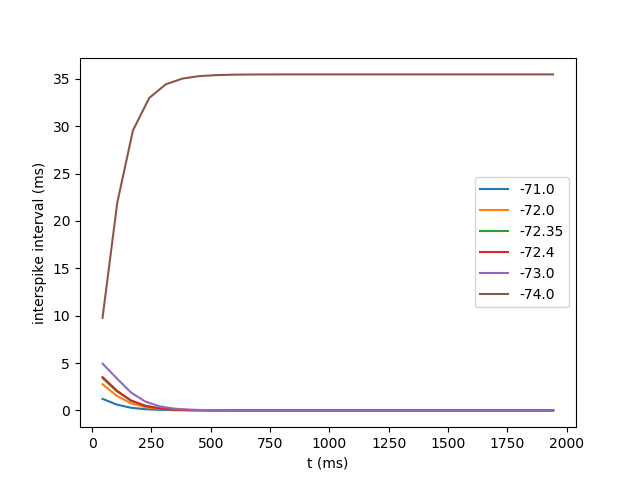
\includegraphics[width = 1.0\linewidth, trim={20 10 20 20}, clip=true]{intervals_ts_13i.png}
		\subcaption{$\tau_s = 13$}
		\label{fig:ts13}	
	\end{subfigure}%
\label{fig:intsi}
\caption{Interspike interval over time for a pair of inhibitory neurons given different $\tau_s$ values. In every case, neuron 1 was initialized at $-70 mV$ and each line corresponds to a different $V_init$ of neuron 2, ranging from $-71$ to $-74 mV$. If a line goes to zero, it indicates that the long term behavior of the system is synchronous firing.}
\end{figure}

We see that for $\tau_s=10ms$ and $V_{init}(1)=-70 mV$, a difference in initial potentials between the two neurons of $-2.35 mV$ leads to long-term synchronous firing while a potential difference larger than $-2.40mV$ leads to alternate firing. We also note that convergence in this case is much quicker than for the excitatory neurons.
How similar the initial potentials must be for synchronous firing depends strongly on $\tau_s$, with shorter time constants requiring more similar initial potentials (figure \ref{fig:ts7}) and longer time constants exhibiting synchronous firing for more dissimilar potentials (figure \ref{fig:ts13}).

Of course we cannot qualitatively investigate plots as the above for every possible set of parameters and initial conditions. Instead, we let $\tau_s \in [5, 10, 15]$ and $r_m \bar g_s \in [0.05, 0.15, 0.30]$ for both excitatory and inhibitory neurons and run 75 simulations for each parameter set with $V_1$ and $V_2$ initialized uniformly at random in $[-55, -80]$.
We then quantify the firing rate and interspike interval at equilibrium for each simulation.
In this case, we run each simulation for $10000 ms$ rather than assessing convergence during the simulation, since this is sufficiently long to ensure convergence for all parameter sets as evident from figure \ref{fig:scat}.

Similarly to the Hodgkin Huxley model, if the time difference between the final two spikes of neuron 1 is $\Delta T$, we calculate the firing rate as $\omega = \dfrac{1}{\Delta T}$ and require the final spike to occur within $\Delta T$ of terminating the simulation.
In this case we also do not need to average over multiple spikes since the simulation is deterministic with no stochastic component.

Scatterplots of the equilibrium quantities for all 75 simulations at each parameter set are given in figure \ref{fig:scat}. The parameter set $(E_s = -80, \tau_s = 0.15, r_m \bar g_s = 0.30)$ is not included since in the case of strong inhibitory synapses with large time constants, the firing of neuron 2 is completely supressed by neuron 1, and only neuron 1 fires.

\begin{figure}[h]
	\centering
	\begin{subfigure}[t]{0.8\linewidth}
		\centering
		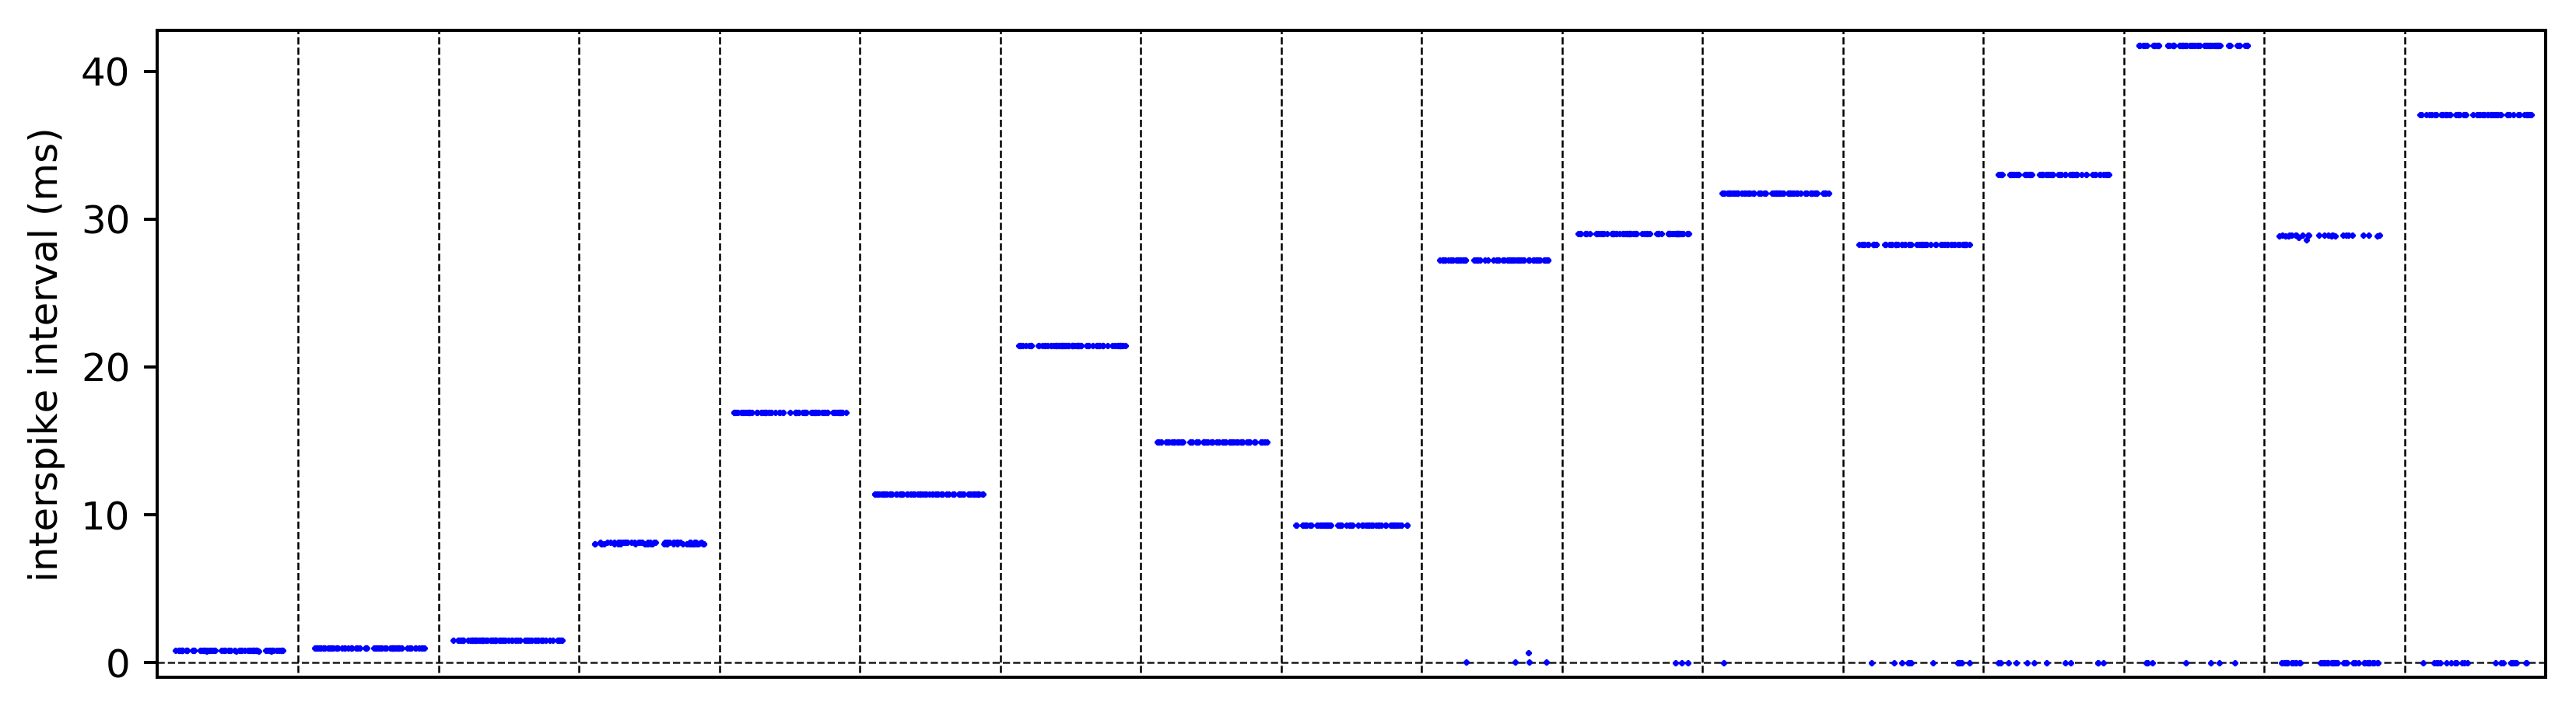
\includegraphics[width = 1.0\linewidth, trim={0 7 0 0}, clip=true]{ints_scatter.png}
		%\subcaption{interval between two neurons firing. for different parameters and random initial conditions}
		\label{fig:int}	
	\end{subfigure}%
	\hspace{0.001\linewidth}
	\begin{subfigure}[t]{0.8\linewidth}
		\centering
		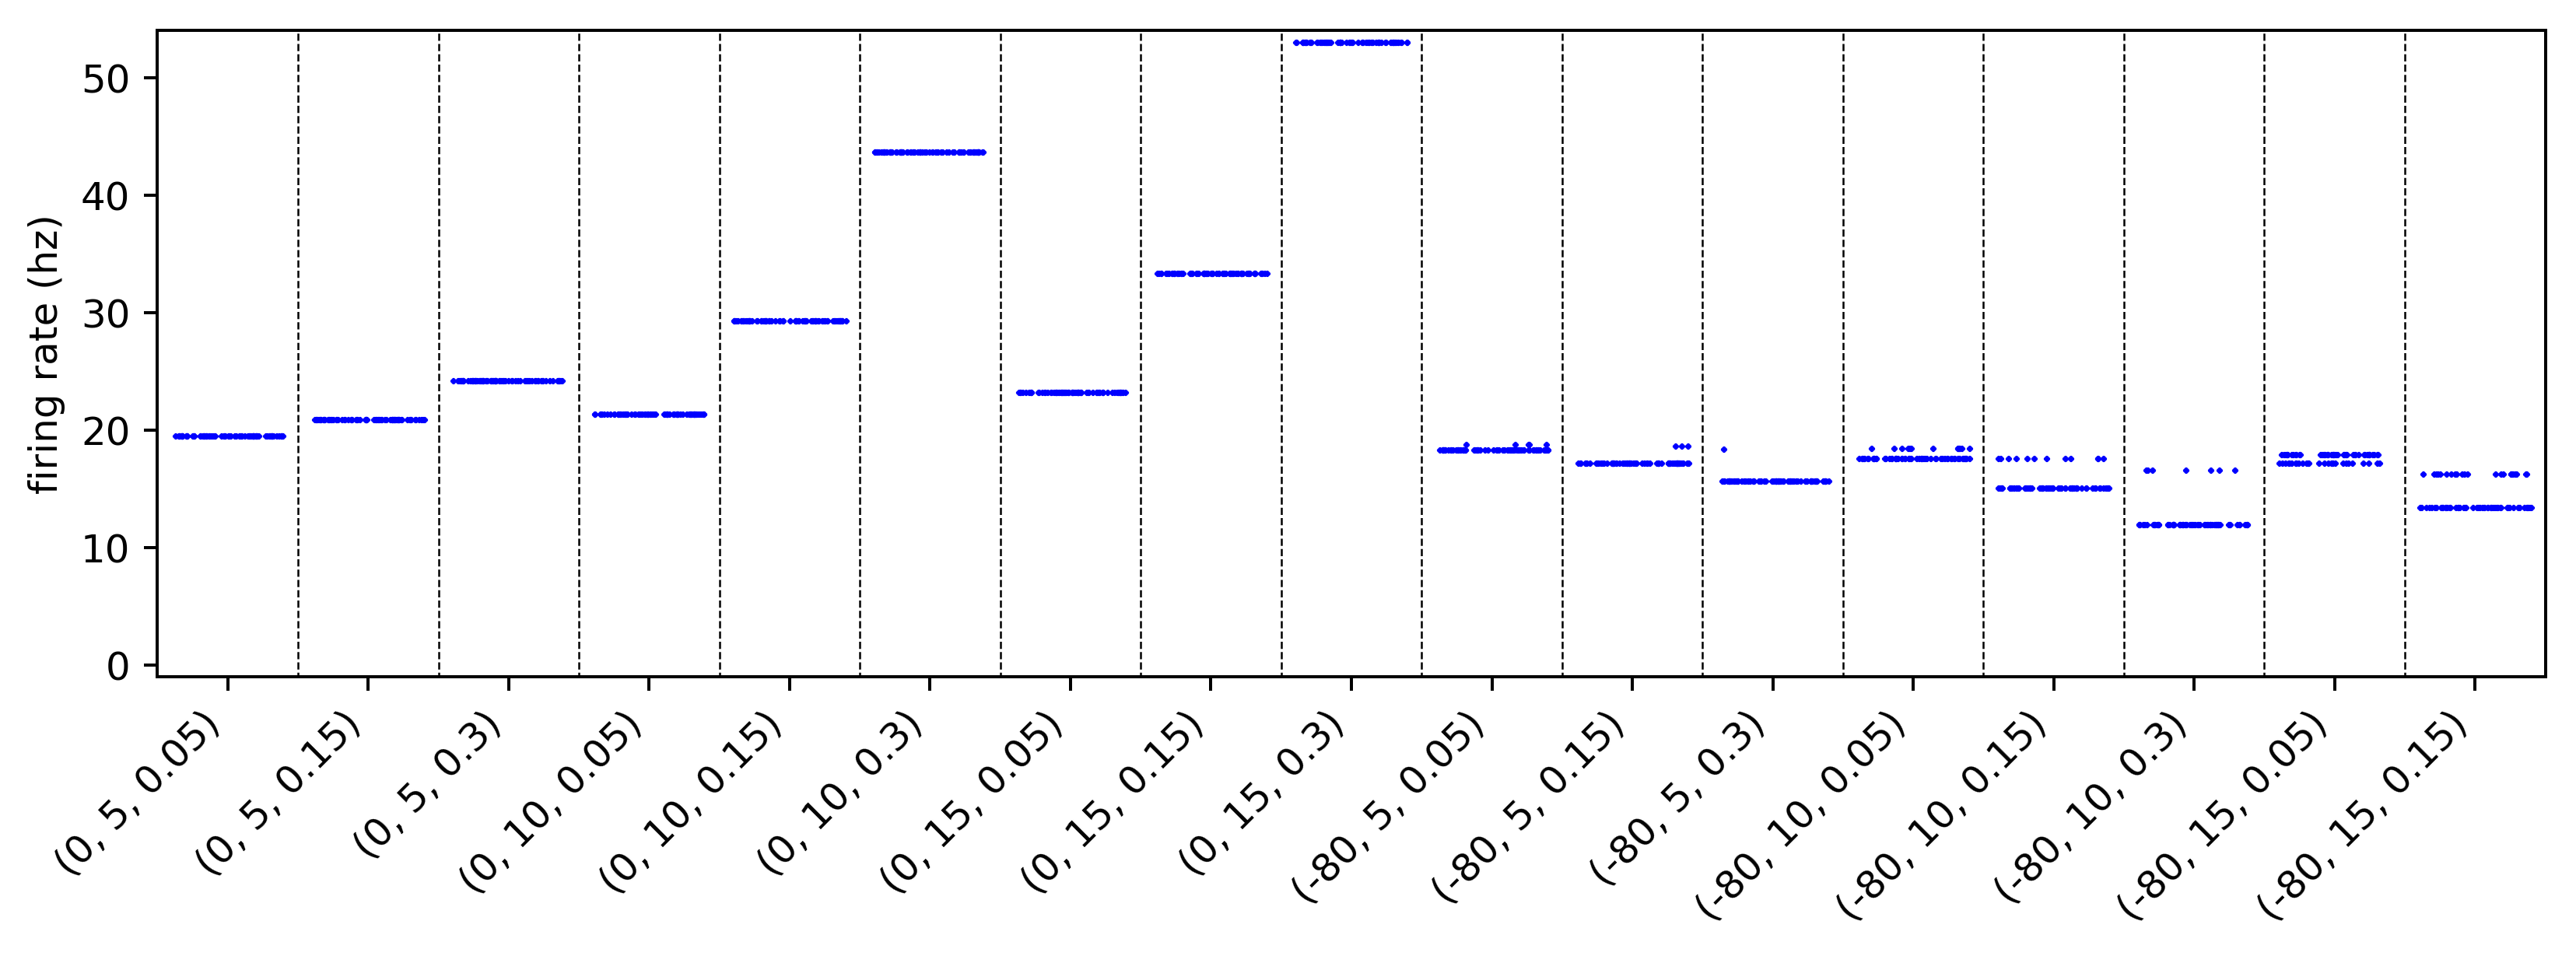
\includegraphics[width = 1.0\linewidth, trim={0 0 0 7}, clip=true]{rates_scatter.png}
		\label{fig:rate}	
	\end{subfigure}%
\label{fig:scat}
\caption{Firing rate (bottom) and interspike interval (top) for 75 simulations at different initial conditions for a range of parameter sets specified using the notation $(E_s, \, \tau_s, \, r_m \bar g_s)$. Whenever the dots split into two distinct groups, the long term behavior depends on the initial state of the system with one group corresponding to synchronous firing (interspike interval of zero) and one to alternate firing.}
\end{figure}

We see from figure  \ref{fig:scat} that the long term behavior of an excitatory system is completely determined by the physical parameters and is independent of initial conditions. We find that the equilibrium firing rate increases with both $\tau_s$ and $r_m \bar g_s$ as discussed above, and that the firing of our two neurons becomes increasingly less synchronous with $\tau_s$ and $r_m \bar g_s$. Note that while the interspike interval decreases e.g. from $(0,10,0.05)$ to $(0,10,0.15)$, this still corresponds to more synchronous firing due to the increase in firing rate. For the $(0,5,0.05)$ system, firing is almost synchronous, with neuron 1 driving firing of neuron 2 shortly afterwards.

However, this near-synchronous behavior is fundamentally different from the behavior of inhibitory neurons where we can observe firing patterns that are \textit{exactly} synchronous in the long time limit. We see that the proportion of synchronous firing increases with $\tau_s$ but decreases with $r_m \bar g_s$ as discussed above. However, while the frequency of synchronous firing decreases with $r_m \bar g_s$, the difference in firing rate between alternate firing and synchronous firing increases with $r_m \bar g_s$ since the stronger synapses lead to stronger inhibition between the alternately firing neurons and thus a relatively lower firing rate.


\section{Networks}

It is common to separate the neurons of a network model into a population of excitatory neurons and a population of inhibitory neurons, allowing us to describe the time evolution of the network by two differential equations

\begin{equation}
\tau_E \dfrac{dv_E}{dt} = -v_E + [M_{EE}v_E+M_{EI}v_I-\gamma_E]_+
\end{equation}

\begin{equation}
\tau_I \dfrac{dv_I}{dt} = -v_I + [M_{IE}v_E+M_{II}v_I-\gamma_I]_+
\end{equation}

Here, $\gamma$ is an external input which could be e.g. a previous layer of neurons. $M_{AB}$ specifies the input from population $B$ to population $A$, and given the division into inhibitory and excitory neurons, we require $M_{AI} \leq 0$ and $M_{AE} \geq 0$. In the present case we describe the excitatory and inhibitory populations by a single firing rate each, but we could expand the firing rates of each individual neuron, which would also require all $M_{AB}$ to be matrices corresponding to potentially variable connectivity.

The partition into excitatory and inhibitory neurons allows us to easily satisfy Dale's law stating that a presynaptic neuron cannot activate some postsynaptic neurons and inhibit others. This follows from the fact that most characterized neurons release only a single major neurotransmitter, and that a neurotransmitter is generally either excitatory or inhibitory in mammals. Exceptions exist in other organisms, with e.g. acetylcholine having both excitatory and inhibitory receptors in \textit{Drosophila melanogaster}.

We can easily find the nullclines of equations 9 and 10 by setting the lefthand side of each equation equal to zero, which gives
\begin{equation}
v_E = \dfrac{\gamma_E-M_{EI} v_I}{M_{EE}-1} = \dfrac{\gamma_E}{M_{EE}-1}-\dfrac{M_{EI}}{M_{EE}-1} v_I
\end{equation}

\begin{equation}
v_I = \dfrac{ \gamma_I - M_{IE} v_E}{M_{II}-1} = \dfrac{\gamma_I}{M_{II}-1} - \dfrac{M_{IE}}{M_{II}-1} v_E 
\end{equation}

This tells us where the gradient of each firing rate is zero, and these nullclines are plotted in figure \ref{fig:nulls}.
We can also rewrite the expression for $v_I$ nullcline to give $v_E$ as a function of $v_I$ and find the fixed point of this system as the intersection of the two nullclines.

\begin{equation}
v_E = \dfrac{\gamma_I}{M_{IE}} - \dfrac{M_{II}-1}{M_{IE}} v_I 
\end{equation}

This gives

\begin{equation}
v_{I,fp} =    ( \dfrac{\gamma_E}{M_{EE}-1} - \dfrac{\gamma_I}{M_{IE}} ) / (\dfrac{M_{EI}}{M_{EE}-1} -  \dfrac{M_{II}-1}{M_{IE}})  
\end{equation}

To determine wheter this fixed point is stable of unstable, we can investigate the eigenvalues of the Jacobian of equations 9 and 10 evaluated at the fixed point, corresponding to the Hessian of $(v_E, v_I)$ which tells us about the behavior of the system near the minimum.

\[
J = 
\begin{bmatrix}
   \dfrac{M_{EE}-1}{\tau_E} &  \dfrac{M_{EI}}{\tau_E} \\
     \dfrac{M_{IE}}{\tau_I} & \dfrac{M_{II}-1}{\tau_I} \\
\end{bmatrix}
\]

The eigenvalues of this matrix are given by

\begin{equation}
\lambda = \dfrac{1}{2}[\dfrac{M_{EE}-1}{\tau_E}+\dfrac{M_{II}-1}{\tau_I} \pm \sqrt{(\dfrac{M_{EE}-1}{\tau_E}+\dfrac{M_{II}-1}{\tau_I})^2 + \dfrac{4M_{EI}M_{IE}}{\tau_E \tau_I}}]
\end{equation}

Armed with these equations, we can begin to characterize our system of interest given a set of physical parameters.
In the following we vary $\tau_I$ and use fixed parameters given in table \ref{tab:paramsnet}

\begin{table}[h]
\centering
\begin{tabular}{ |c|c|c|c|c|c|c|}
\hline
 $M_{EE}$ & $M_{IE}$ & $M_{EI}$ & $M_{II}$ & $\gamma_E$ & $\gamma_I$ & $\tau_E$\\
\hline
$1.25$ & $1$ & $-1$ & $-1$ & $-10 Hz$ & $10 Hz$ & $10 ms$\\
\hline
\end{tabular}
\caption{Fixed parameters in the network model}
\label{tab:paramsnet}
\end{table}

Together with the equations above, this gives the coordinates of the single fixed point of the system as $v_{I,fp} = 25$ and $v_{E,fp} = 60$. 

We further plot the real parts of the eigenvalues of the Jacobian in figure \ref{fig:ti}. Dynamical systems theory tells us that the system will be stable if $\Re{\lambda_1}, \Re{\lambda_1} < 0$. The fixed point will be unstable if the real part of at least one eigenvalue is positive. Higher order derivatives must be considered if the real part of the largest eigenvalue is exactly zero.
%
%We first find find the limiting values $\lambda_i$ as $\tau_I$ tends to $0$ and $\inf$. As $\tau_I$ tends to $0$ we Taylor expand the squareroot and only include the lowest the highest order term in \ $\dfrac{1}{\tau_I}$. This gives
%
%\begin{equation}
%\lambda_0 = (0.5\dfrac{M_{EE}-1}{\tau_E}, 0.5\dfrac{M_{EE}-1}{\tau_E} + \dfrac{M_{II}-1}{\tau_I}) = (0.0125, -\inf)
%\end{equation}
%
%As $\tau_I$ tends to $\inf$ we can ignore all terms including any power of $\dfrac{1}{\tau_I}$. This gives
%
%\begin{equation}
%\lambda_0 = (0, \dfrac{M_{EE}-1}{\tau_E}) = (0, 0.025)
%\end{equation}

We start by finding the values of $\tau_I$ for which the discriminant of equation 15 is 0, which we do by solving the quadratic equation. This gives

\begin{equation}
\lambda_{D=0} = (8.08, 791.92)
\end{equation}

We further find that $\Re{\lambda_1}, \Re{\lambda_2} < 0$ for $\tau_I = 8.08$ and $\Re{\lambda_1}, \Re{\lambda_2} > 0$ for $\tau_I = 791.92$. There must therefore be a transition between a stable and unstable fixed point within the interval of $\tau_I \in [8.08, 791.92]$ corresponding to complex eigenvalues. We can find this transition point by ignoring the squareroot term when setting $\Re{(\lambda_{1})}, \Re{(\lambda_{2} )}= 0$ since this will be imaginary. We thus solve

\begin{equation}
 \dfrac{1}{2}[\dfrac{M_{EE}-1}{\tau_E}+\dfrac{M_{II}-1}{\tau_I} ] = 0
\end{equation}
Which gives

\begin{equation}
\tau_I = \dfrac{\tau_E(1-M_{II})}{M_{EE}-1} = 80 ms
\end{equation}

This is consistent with the graph in figure \ref{fig:ti} which show no other transitions, and we thus conclude that the system has a stable fixed point for all $\tau_I < 80 ms$ and an unstable fixed point for all $\tau_I > 80$.

\begin{figure}[h]
	\centering
	\begin{subfigure}[t]{0.45\linewidth}
		\centering
		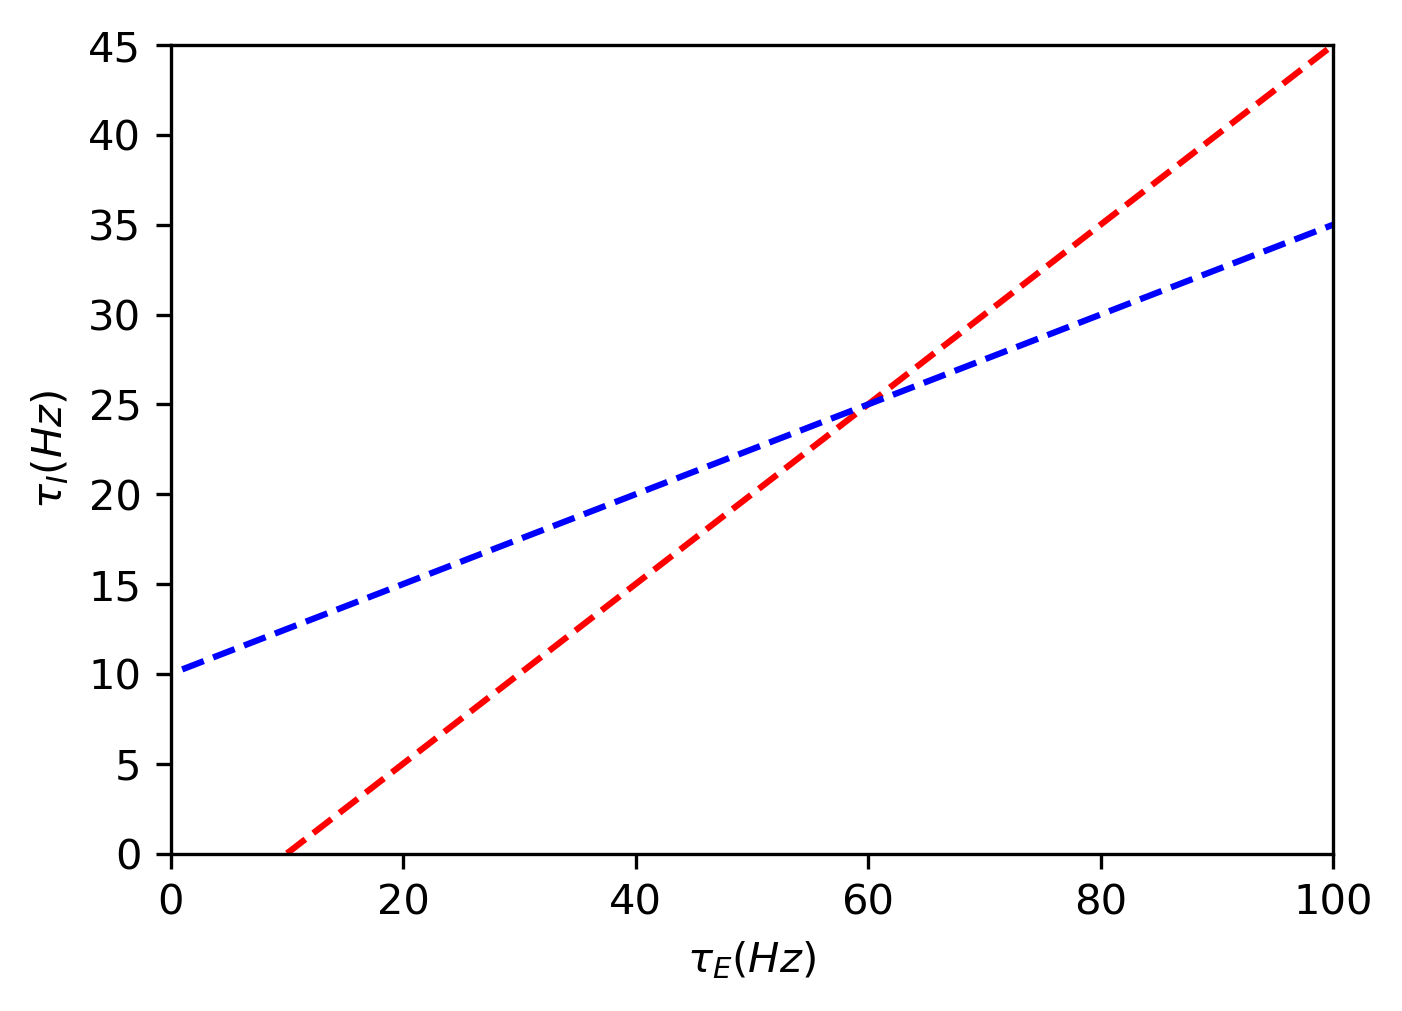
\includegraphics[width = 1.0\linewidth, trim={0 7 0 0}, clip=true]{nullclines.png}
		\subcaption{Nullclines for $v_E$ (blue) and $v_I$ (red) }
		\label{fig:nulls}	
	\end{subfigure}%
	\hspace{0.001\linewidth}
	\begin{subfigure}[t]{0.45\linewidth}
		\centering
		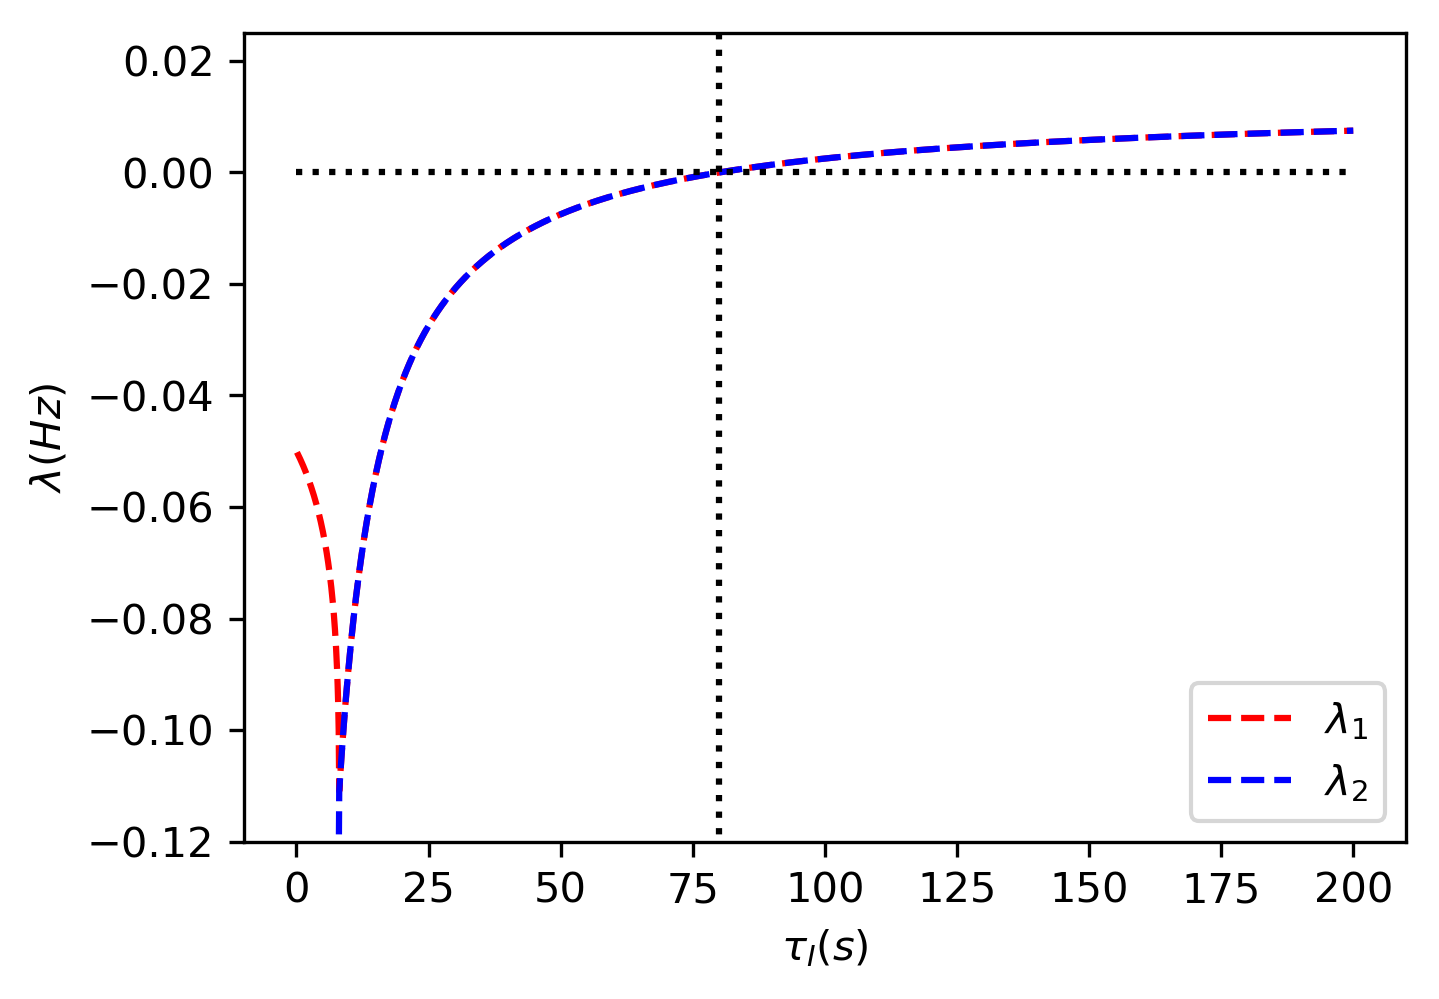
\includegraphics[width = 1.0\linewidth, trim={0 7 0 0}, clip=true]{ti_scan.png}
		\subcaption{Real parts of the eigenvalues of the Jacobian for the network model as a function of $\tau_I$.}
		\label{fig:ti}	
	\end{subfigure}%
\end{figure}

To verify this result, we run a pair of simulations using equations 9 and 10, letting the system evolve over time with $dt=0.01$. The result of simulations with $\tau_I = 75, 85$ are plotted in figure \ref{fig:sims}, projected onto the $(v_I, v_E)$ plane together with the two nullclines as above and a gradient field.



\begin{figure}[h]
	\centering
	\begin{subfigure}[t]{0.45\linewidth}
		\centering
		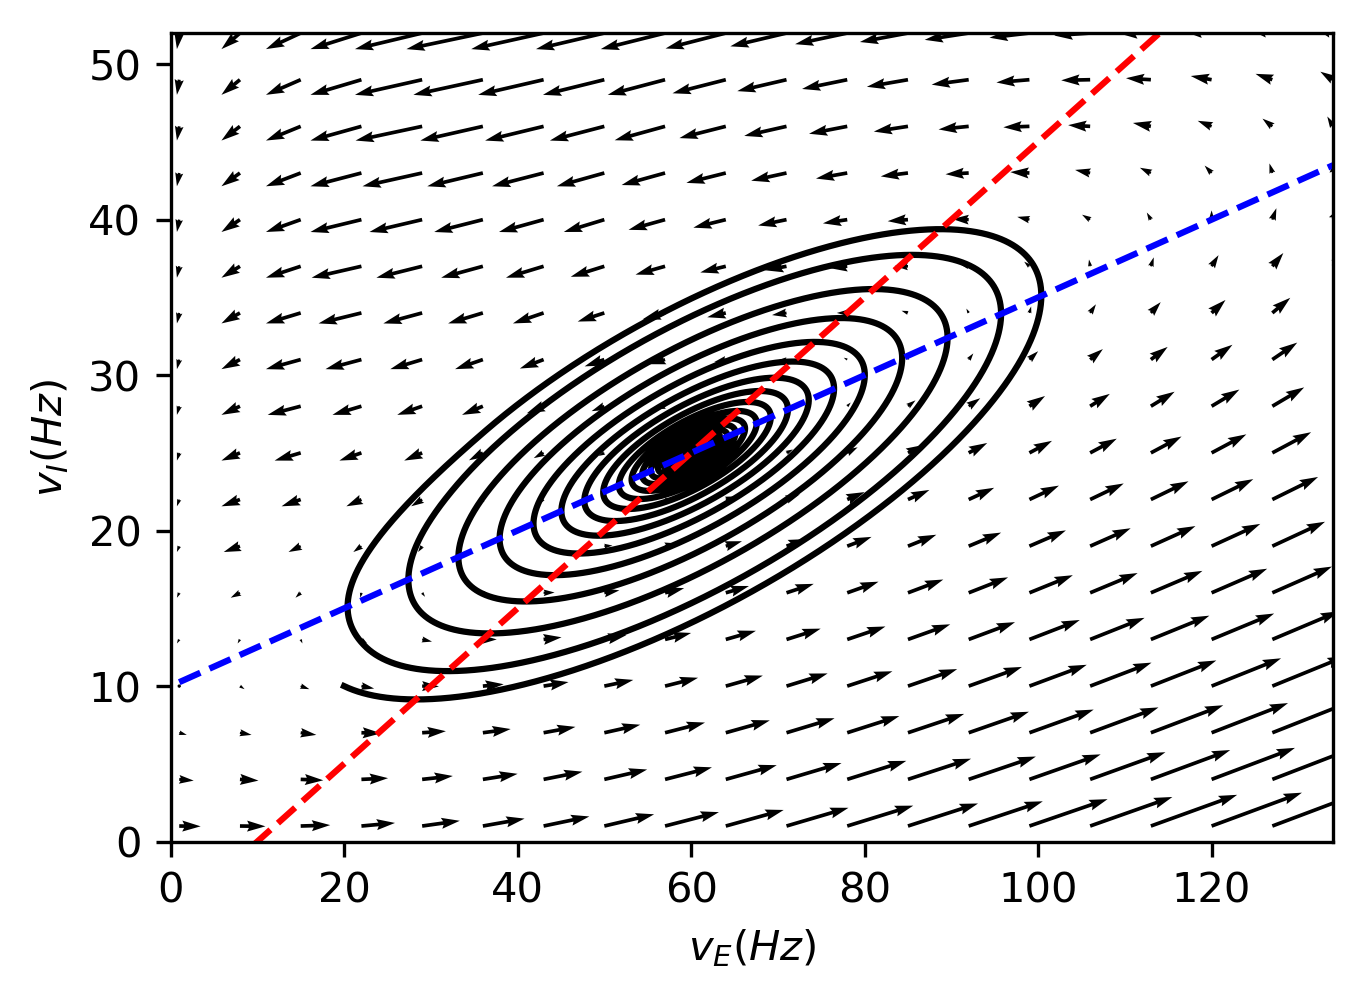
\includegraphics[width = 1.0\linewidth, trim={0 7 0 0}, clip=true]{trajectcon.png}
		\subcaption{}
		\label{fig:con}	
	\end{subfigure}%
	\hspace{0.001\linewidth}
	\begin{subfigure}[t]{0.45\linewidth}
		\centering
		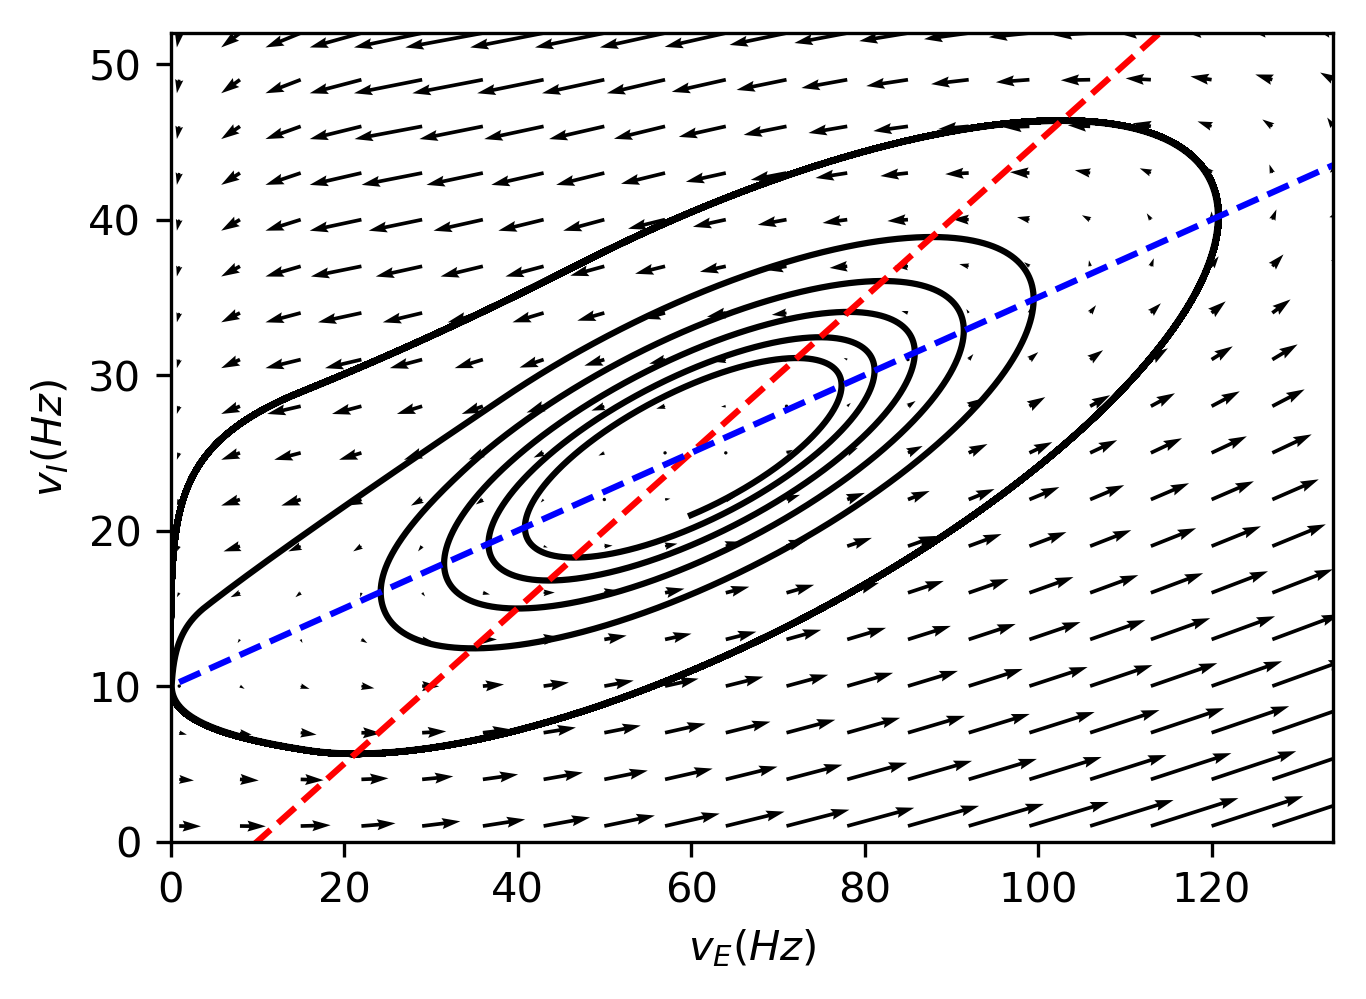
\includegraphics[width = 1.0\linewidth, trim={0 7 0 0}, clip=true]{trajectdiv.png}
		\subcaption{}
		\label{fig:div}	
	\end{subfigure}%
\label{fig:sims}
\caption{Simulation of a network of excitatory and inhibitory neurons with $\tau_I = 75 ms$ (left) or $\tau_I = 85 ms$ (right). The systems were initialized at $(v_E, v_I) = (20 mV, 10 mV)$ and $(v_E, v_I) = (60 mV, 20 mV)$ respectively . We see that the fixed point is stable for $\tau_I = 75 ms$ and unstable for $\tau_I = 85 ms$ }
\end{figure}

The simulation with $\tau_I = 75$ is initiated at $(v_E, v_I) = (20, 10)$ and we see that it converges to the stable fixed point at $(60, 25)$. For the simulation with $\tau_E = 85$, on the contrary, we start the simulation at $(60, 20)$ near the fixed point, but observe a divergence away from the fixed point as it is unstable in this case.

We note that since both simulations have time constants close to $\tau_I = 80$, the gradients near the fixed point are small and convergence is relatively slow near the fixed point for $\tau_I = 75$.

\section{Hopfield network}

In the following, we investigate the properties of a binary hopfield network. Such a network can be described as a fully connected graph with $N$ nodes and reciprocal connections between every pair of nodes given by a weight matrix $W$. Each node can take values -1 or 1. We define the energy of a network with states $V_i$ as

\begin{equation}
E = - \sum_{i>j}{W_{ij}V_i V_j}
\end{equation}

Given this energy function, we can minimize the energy of the network given a fixed weight matrix for a particular set of initial states by updating the states according to

\begin{equation}
V_i(t+1) = \text{sign}(\sum_{j \neq i}{W_{ij}V_j(t)})
\end{equation}

In the present case we update the network asynchronously but iterate through the nodes systematically until the system is stationary. The change in energy for each step is then

\begin{equation}
\Delta E = (V_i(t) - V_i(t+1)) \sum_{j \neq i}{W_{ij}V_j} \leq 0
\end{equation}

This ensures convergence since the energy is bounded from below.


Mackay and others have often used visual representations to underline the ability or inability of a Hopfield network to recall patterns. However, for a fully connected network, the spatial arrangement of nodes is completely arbitrary, and in the following we therefore pursue a more general approach that is easily quantified and thus allows us to cove a large region of parameter space.

We assess the capacity of a network based on its ability to store randomly generated patterns. We train the network on $n_{pat}$ patterns $V^s$ with states $V^s_i$ by setting the weights according to
\begin{equation}
W_{ij} = \dfrac{1}{N} \sum_s{V_i^s V_j^s}
\end{equation}
i.e. the strength of a connection from $i$ to $j$ is given by the fraction of patterns in which neurons $i$ and $j$ are in the same state minus the fraction of patterns in which their states differ. This can be interpreted as a simple form of Hebbian learning where the strength of a synapse increases the more co-active they are.

To assess the recall of the network, we then select a random sample of 100 learned patterns, for each of these we reverse a fraction $f_{err}$ of the states, and we then compare the pattern converged to from this initial state to the original learned pattern. This corresponds to assessing associative recall given $1-2*f_{err}$ of the original information. The factor of two arises because reversing half the states leads to a complete lack fo correlation whereas reversing all states leads to perfect anticorrelation. We further define an error function between the learned pattern and the converged pattern as 

\begin{equation}
\epsilon = 1 - \dfrac{v_{learned}\cdot v_{converged}}{N}
\end{equation}

For two random vectors $v_{learned}$ and $v_{converged}$, the expected value of the dot product is zero. Our error function thus in theory runs from 0 to 2 if the two vectors are perfectly anticorrelated, but in practice from 0 to 1 where an error of 1 corresponds to no correlation between the learned and converged patterns.

Given this error function, we start by investigating the performance of assocative recall as a function of the fraction of withheld information $f_{err}$. We do this by scanning the error landscape over the number of learned patterns and $f_{err}$, quantifying the error as the mean value of $\epsilon$ when training 10 independent networks for a given parameter set and recalling a sample of 100 learned patterns for each network.
To begin with, we fix the number of nodes at $N = 300$ as this is not expected to significantly influence the effect of $f_{err}$ for large $N$. The result is given in figure \ref{fig:ferr}.

We see that for $f_{err} < 0.12$,  the error for a given number of learned patterns only decreases slightly with $f_err$, with catastrophic forgetting occurring at approximately 50 memorized patterns corresponding to $\dfrac{n_{pats}}{N} = 0.167$. This is illustrated in figure \ref{fig:ferr_thresh} where the maximum capacity for each $f_{err}$ is plotted. In this case, the capacity is defined as the number of learned patterns for which $\epsilon < 0.20$. Defining the capacity as the point of inflection for a given $f_{err}$ gives a similar but noiser result.

Based on these results, we fix $f_{err} = 0.1$ for the remainder of this report, corresponding to assessing associate recall given $80\%$ of the original data. At $f_{err} > 0.25$, the error rapidly goes to a threshold value of $0.8$ even for small numbers of learned patterns suggesting faulty recall given less than 50\% of the original data.

\begin{figure}[h]
	\centering
	\begin{subfigure}[t]{0.50\linewidth}
		\centering
		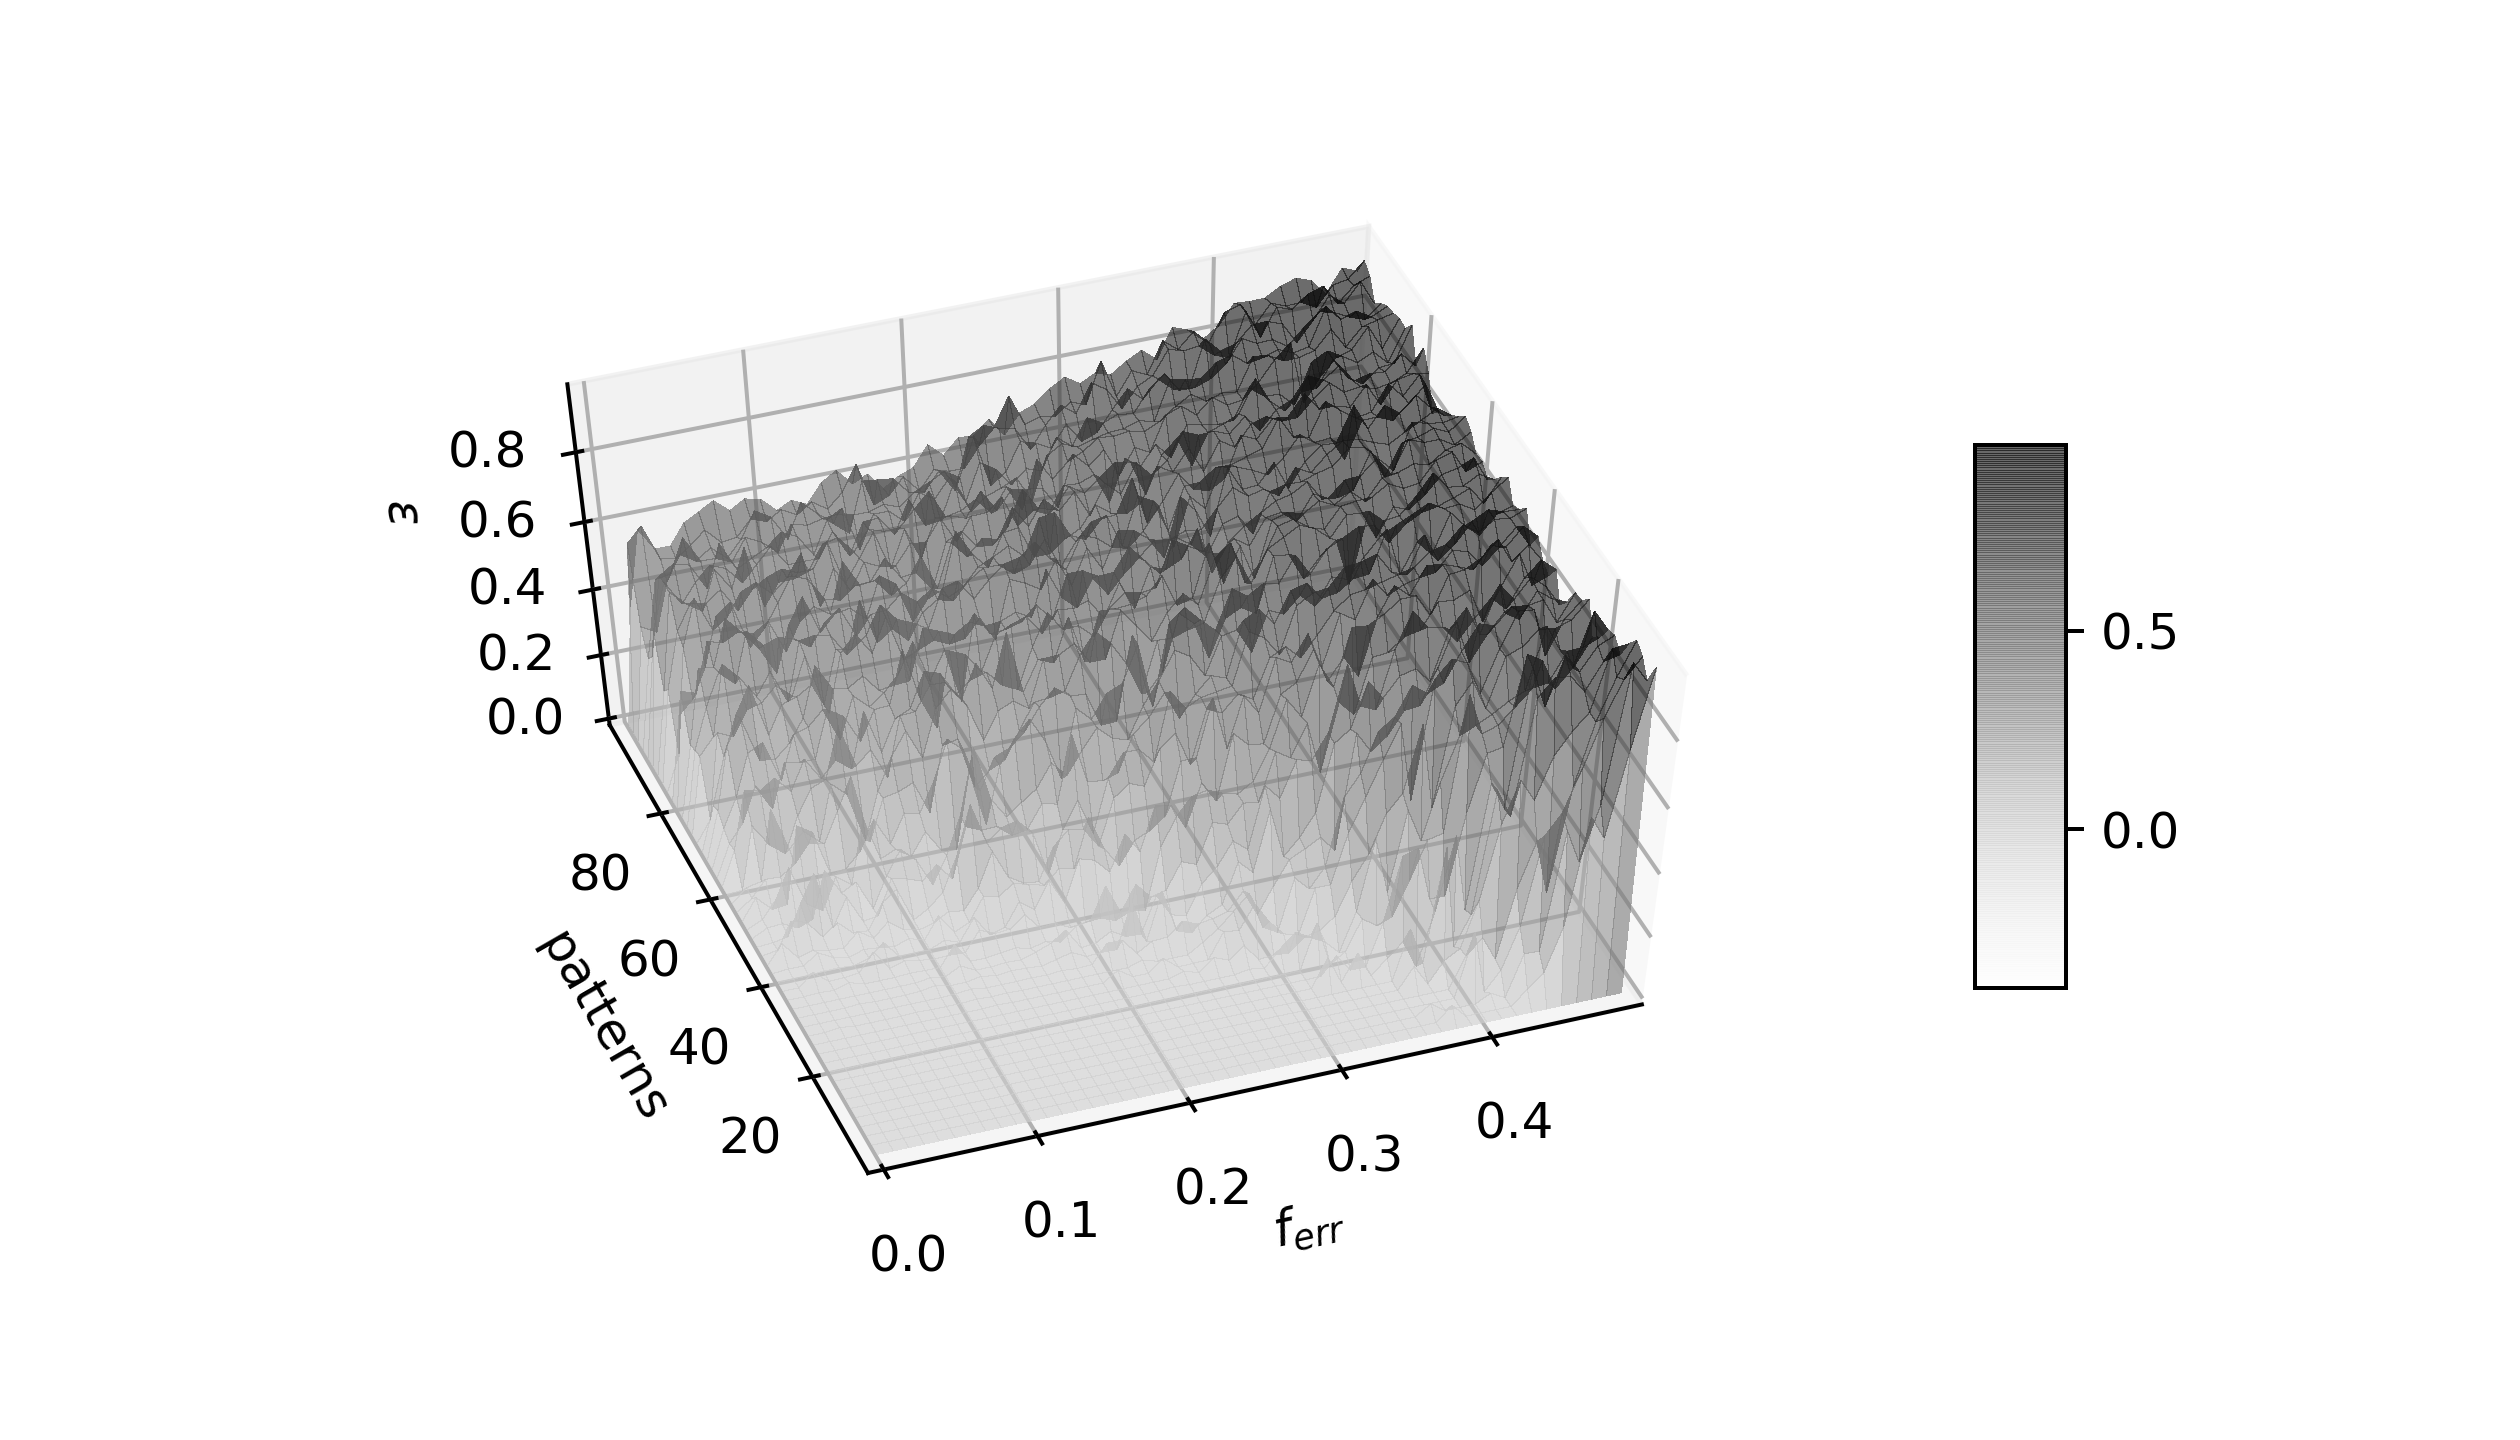
\includegraphics[width = 1.0\linewidth, trim={90 30 50 45}, clip=true]{scan_ferr_npat.png}
		%\subcaption{interval between two neurons firing. for different parameters and random initial conditions}
		\label{fig:ferr}	
	\end{subfigure}%
	\hspace{0.001\linewidth}
	\begin{subfigure}[t]{0.45\linewidth}
		\centering
		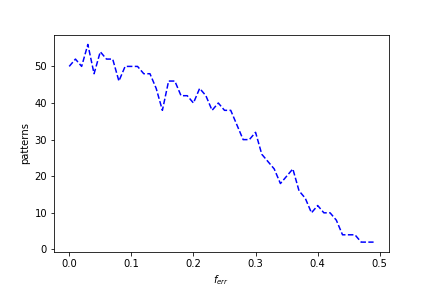
\includegraphics[width = 1.0\linewidth, trim={0 0 0 0}, clip=true]{ferr_thresh.png}
		%\subcaption{interval between two neurons firing. for different parameters and random initial conditions}
		\label{fig:ferrthresh}	
	\end{subfigure}
	\caption{(\textit{left}) error metric $\epsilon$ for recall of a given number of learned patterns with a fraction $f_{err}$ of states reversed for a network of N=300 nodes. (\textit{right}) capacity of the network as a function of $f_{err}$, with the capacity defined as the number of patterns learned before $\epsilon > 0.2$.}
\end{figure}

Given the methodology described above for assessing the properties of a given Hopfield network, we proceed to investigate how the error rate varies as a function of the number of nodes N and the number of learned patterns (figure \ref{fig:Nsamp}).

\begin{figure}[h]
	\centering
	\begin{subfigure}[t]{0.50\linewidth}
		\centering
		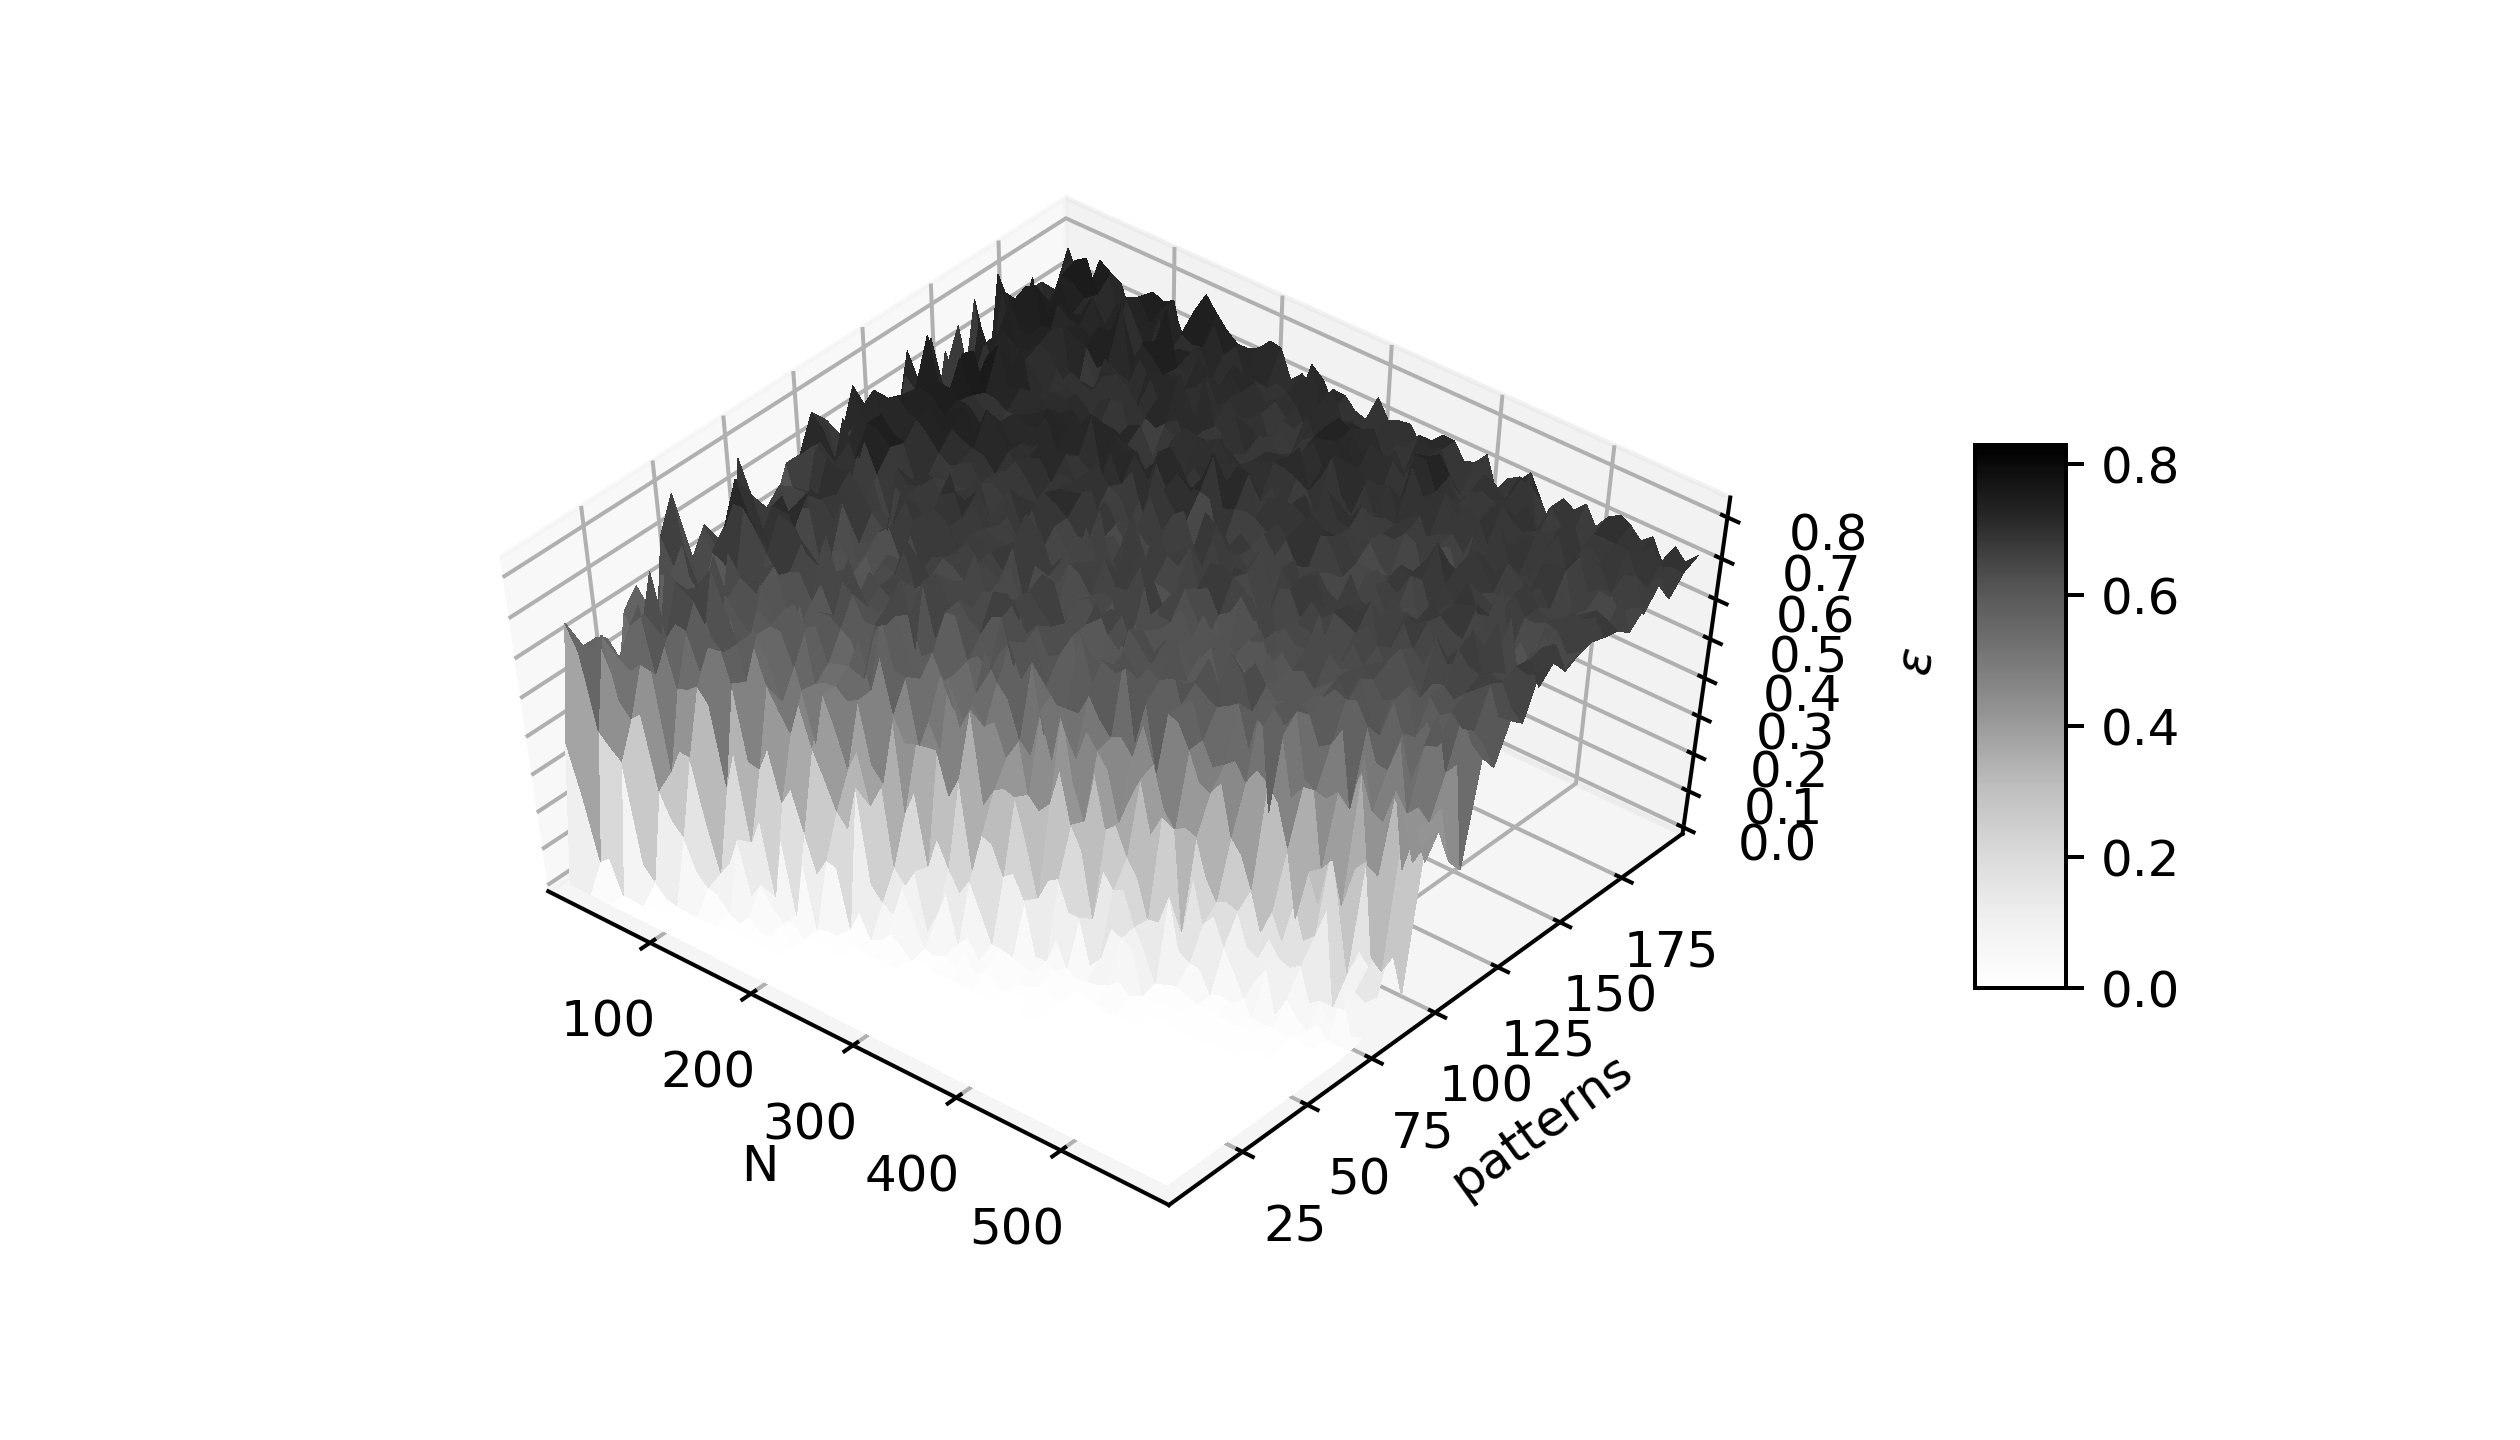
\includegraphics[width = 1.0\linewidth, trim={100 30 50 40}, clip=true]{scan_N_npat.png}
		\label{fig:N}	
	\end{subfigure}%
	\hspace{0.001\linewidth}
	\begin{subfigure}[t]{0.45\linewidth}
		\centering
		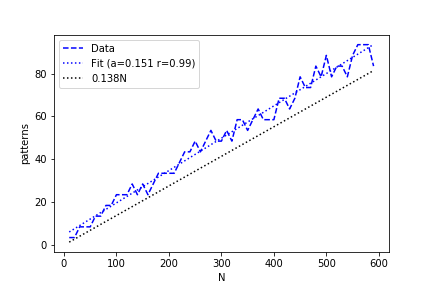
\includegraphics[width = 1.0\linewidth, trim={0 7 0 0}, clip=true]{hebb_thresh.png}
		\label{fig:Nthresh}	
	\end{subfigure}%
\caption{(\textit{left}) error metric $\epsilon$ for recall of a given number of learned patterns for hopfield networks of size N with $f_{err} = 0.1$. (\textit{right}) capacity of the network as a function of N, with the capacity defined as the number of patterns learned before $\epsilon > 0.2$.  Black dotted line corresponds to the Amit et al. model of a capacity of 0.138N. }
\label{fig:Nsamp}
\end{figure}

We see that there is a plateau of perfect recall followed by a rapid transition to an asymptotic error of $\epsilon = 0.8$. The reason the error does not go to 1 is that a given query pattern is likely to converge to an energy minimum that is similar to the query, which will in turn also be similar to the original learned pattern. We find that the capacity of the network as a funciton of N follows an approximately straight line ($r=0.99$) with a slope of $a=0.151$. This corresponds to a slightly higher capacity than that described by Amit et al (1985), but a qualitatively very similar empirical result to their theoretical considerations yielding a capacity of $n_{pat} = 0.138 N$.

We now proceed to vary the sparseness $\alpha$ of the learned patterns with $\alpha$ defined as the probability that a given node is $+1$ in a pattern.
If we query our trained network with a random pattern of sparseness $\alpha$, we expect the normalized dot product with an uncorrelated pattern of sparseness $\alpha$ to be
\begin{equation}
\tilde s = \alpha^2+(1-\alpha)^2-2\alpha(1-\alpha)
\end{equation}

For $\alpha=0.5$, $\tilde s = 0$. however for $\alpha>0.5$, this dot product is greater than zero which should be taken into account in our error function. We therefore define a modified error function as 

\begin{equation}
\epsilon = \dfrac{1}{1-\tilde s} - \dfrac{v_{train}\cdot v_{state}}{N(1-s)}
\end{equation}

Ignoring the effect of introducing a $f_{err}$ errors in our query pattern which slightly reduces the expected value of $\tilde s$, this error metric goes from 0 when $v_{train} = v_{state}$ to 1 when they are both random vectors of sparseness $\alpha$. Note that this expression simplifies to our previous error function when $\alpha=0.5$ corresponding to random assignment of positive and negative states.

We plot in figure \ref{fig:alpha} our new error as a function of the sparseness $\alpha$ of the network and the number of patterns learned for N=300. We see that the capacity of the network decays rapidly with $\alpha$ and is effectively 0 at $\alpha = 0.7$. This is because the difference between patterns becomes smaller and minima start coalescing, leading to faulty recall.

\begin{figure}[h]
	\centering
	\begin{subfigure}[t]{0.44\linewidth}
		\centering
		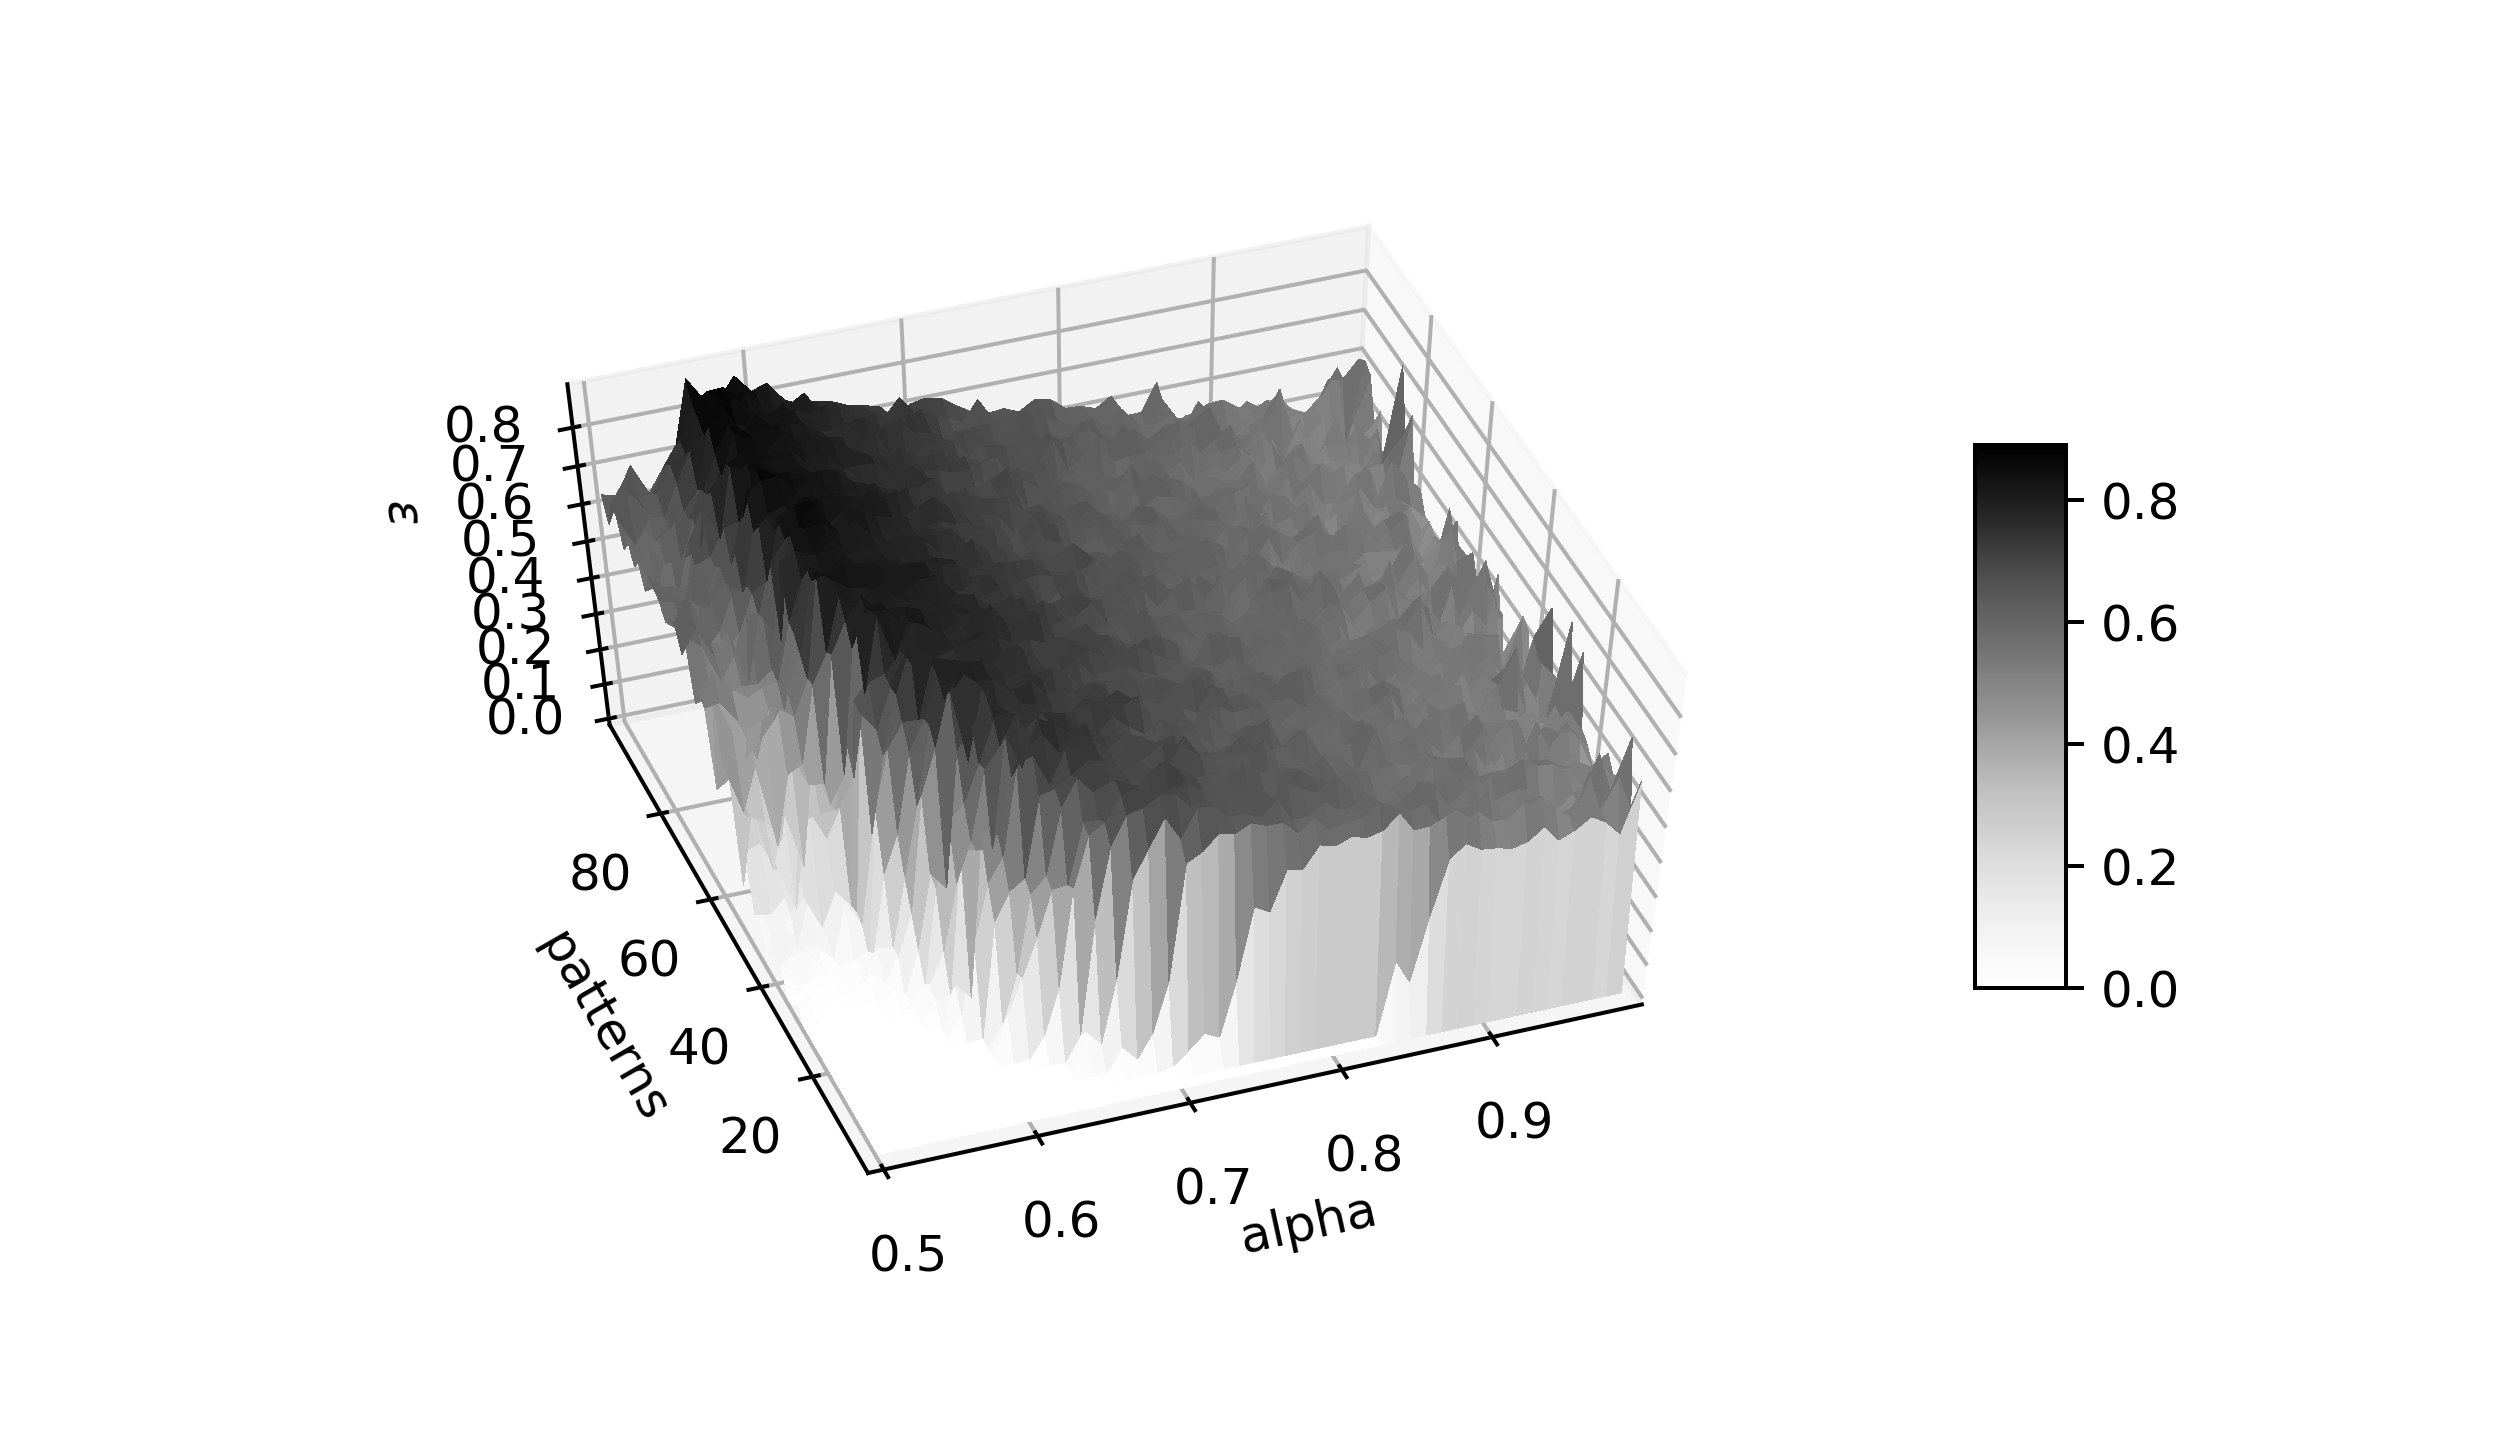
\includegraphics[width = 1.0\linewidth, trim={90 30 50 40}, clip=true]{scan_alpha_npat.png}
		\subcaption{error metric $\epsilon$ for recall of a given number of learned patterns for hopfield networks with different sparesness $\alpha$ for N=300 and $f_{err} = 0.1$.}
		\label{fig:alpha}	
	\end{subfigure}%
	\hspace{0.05\linewidth}
	\begin{subfigure}[t]{0.44\linewidth}
		\centering
		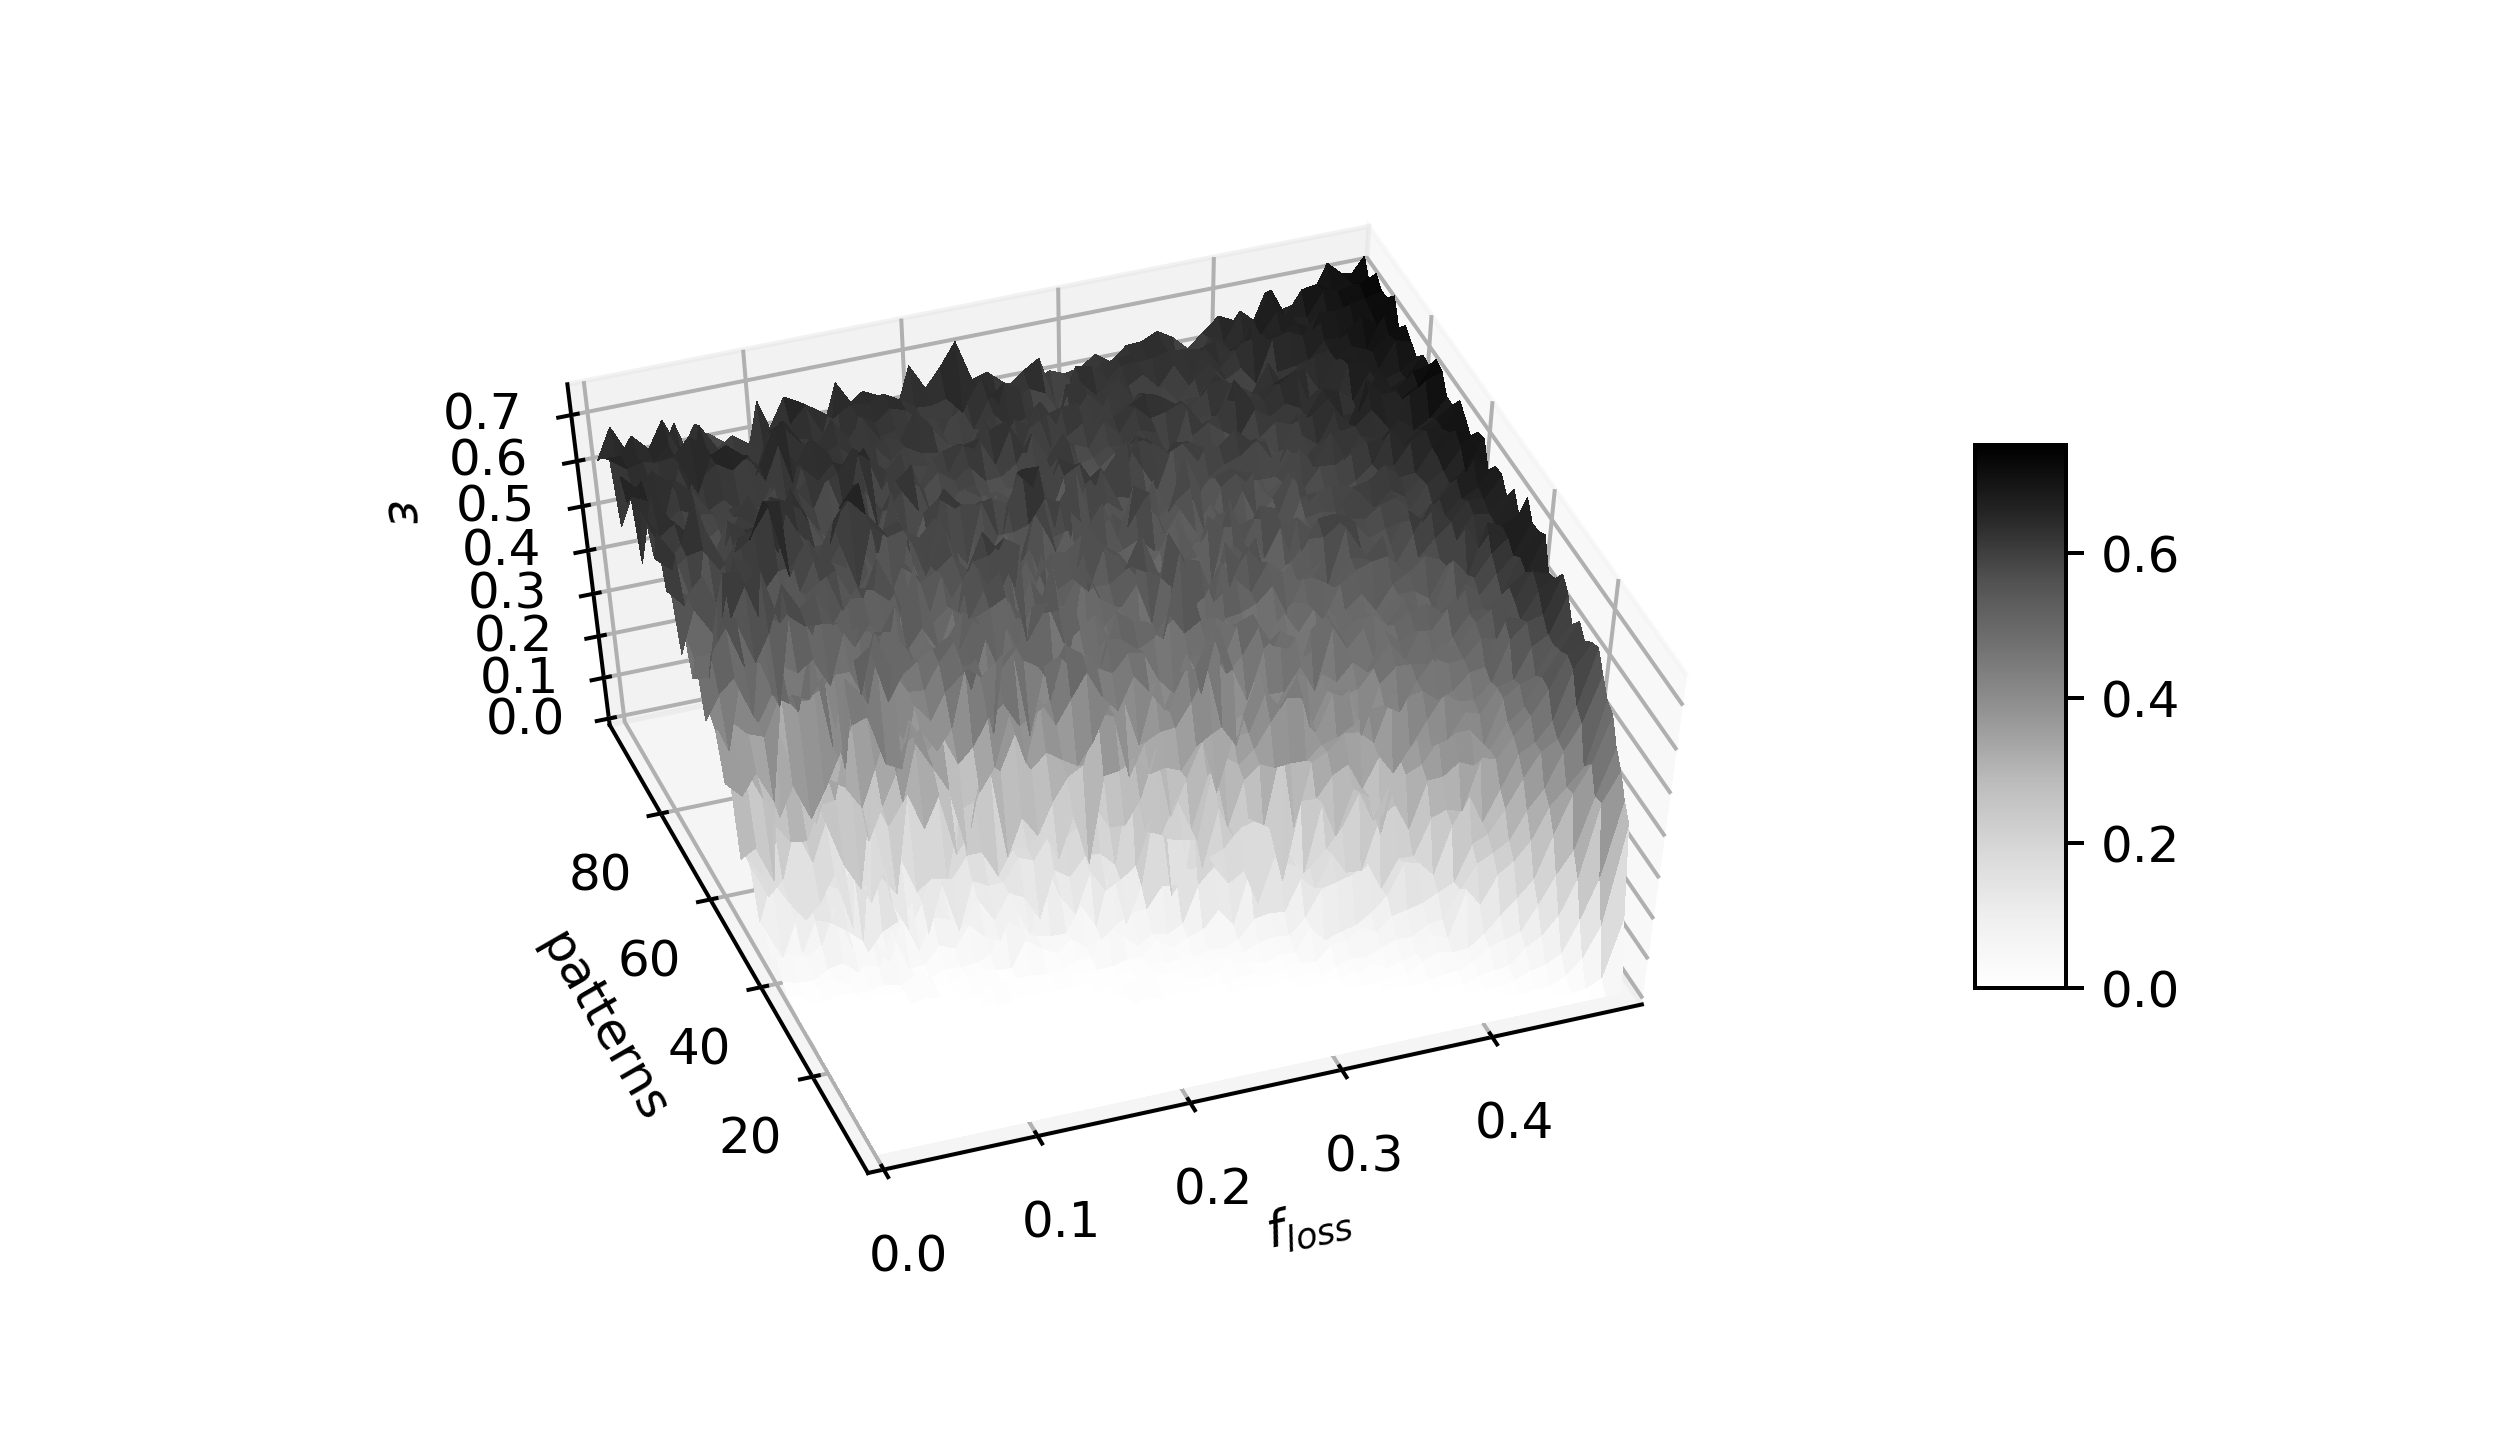
\includegraphics[width = 1.0\linewidth, trim={90 30 50 40}, clip=true]{scan_floss_npat.png}
		\subcaption{error metric $\epsilon$ for recall of a given number of learned patterns for hopfield networks with random loss of a fraction $f_{loss}$ of its weights for N=300 and $f_{err} = 0.1$.}
		\label{fig:floss}	
	\end{subfigure}%
\end{figure}

We can also invetigate the robustness of the network by setting a random fraction $f_{loss}$ of the weights to zero after training (figure \ref{fig:floss}). We see that the network is remarkably robust, retaining 80\% of it's capacity even when losing 20\% of its weights.

\begin{figure}[h]
	\centering
	\begin{subfigure}[t]{0.44\linewidth}
		\centering
		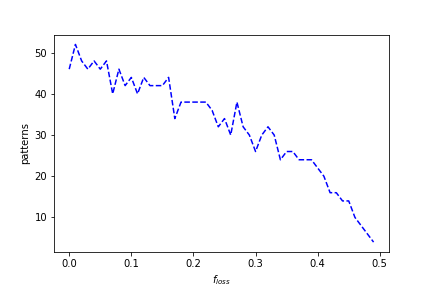
\includegraphics[width = 1.0\linewidth, trim={0 0 0 0}, clip=true]{floss_thresh.png}
		\subcaption{capacity as a function of $f_{loss}$ for $N=300$ and $f_{err}=0.1$.}
		\label{fig:flossthresh}	
	\end{subfigure}%
	\hspace{0.05\linewidth}
	\begin{subfigure}[t]{0.44\linewidth}
		\centering
		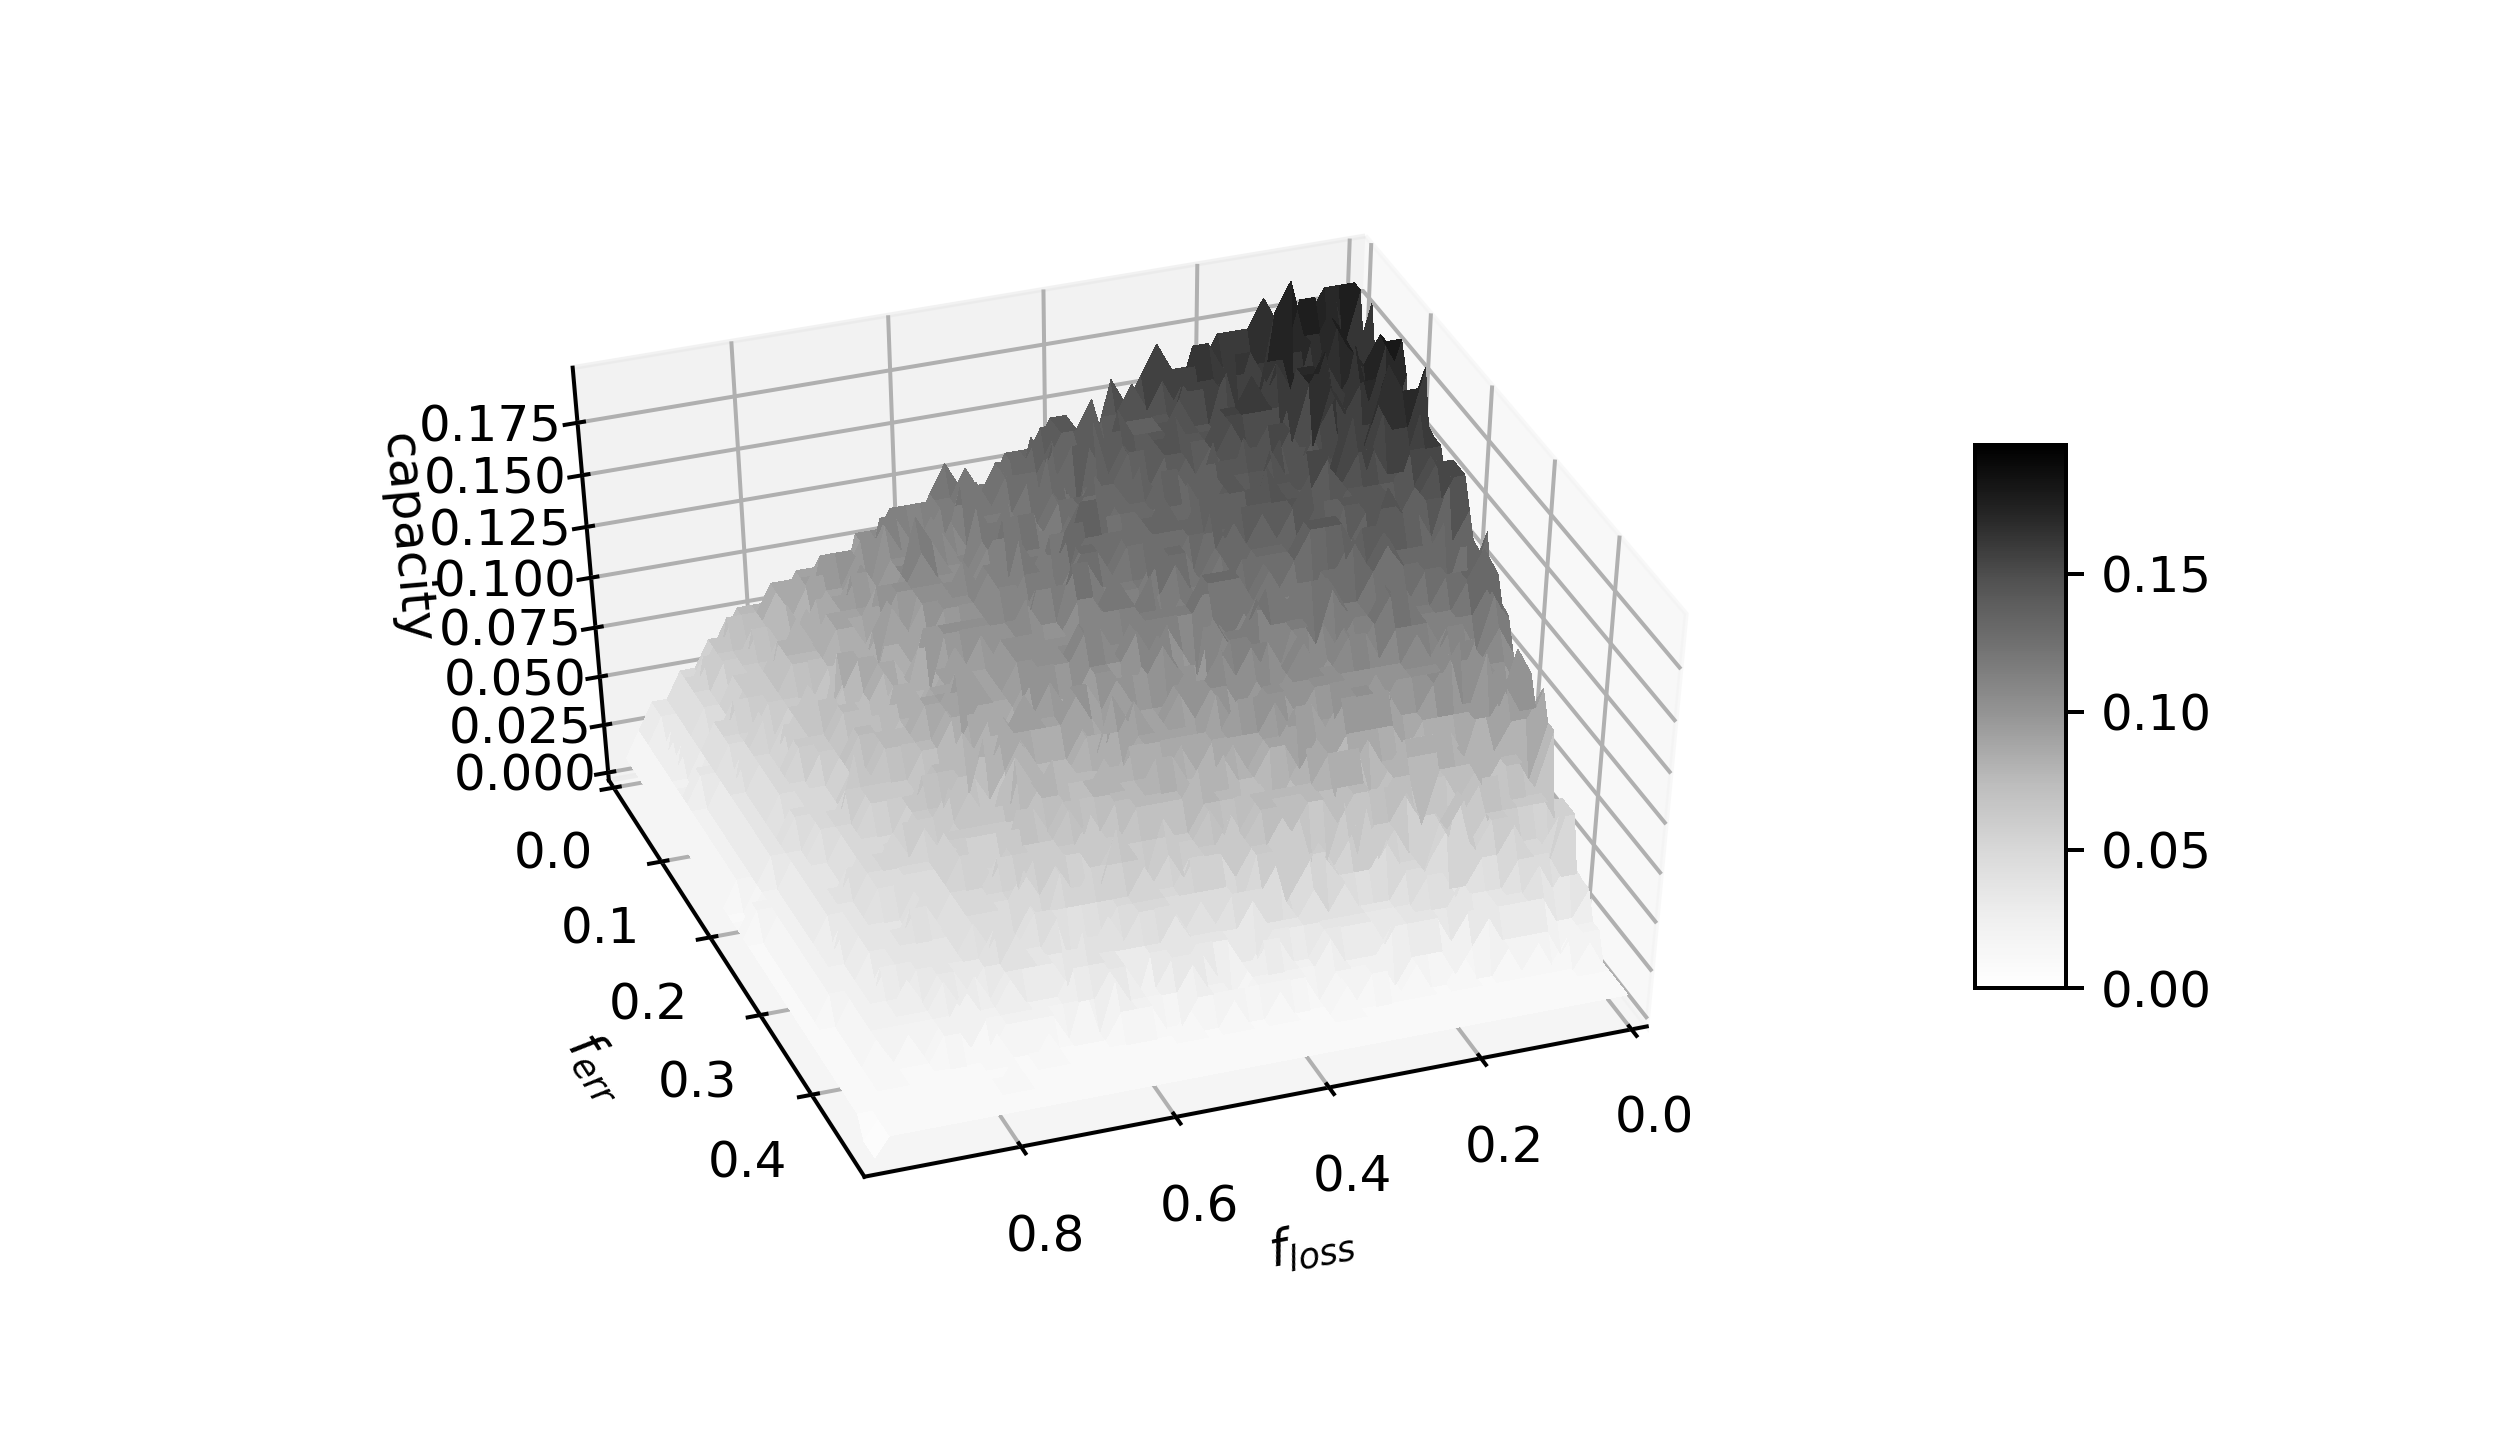
\includegraphics[width = 1.0\linewidth, trim={90 30 50 40}, clip=true]{test_err_loss.png}
		\subcaption{Capacity of the network as a function of $f_{loss}$ and $f_{err}$.}
		\label{fig:cap}	
	\end{subfigure}%
\end{figure}

However, it has been previously shown that Hebbian learning does in fact not optimize the storage capacity of our network. Instead, we can train our network by performing steepest descent on an error function of the learned patterns in a discretized version of the continuous method given in Mackay (algorithm 42.9). This is incidentally also equivalent to the perceptron learning rule introduced in the Deep Learning lectures.

Denoting our input data as $X_{k}^\mu$ for element k of pattern $\mu$, we aim to minimize the error introduced through a single hopfield update step (equation 20). We can find the predicted data for a single Hopfield update step as $T_k^\mu = f(\sum_j{X_j^\mu W_{jk}})=\text{sign}(\sum_j{X_j^\mu W_{jk}})$. This allows us to define an error function

\begin{equation}
E =\sum_{k, \mu}{\dfrac{1}{2}(X_{k}^\mu-T_k^\mu)^2}
\end{equation}
This gives
\begin{equation}
\dfrac{dE}{dW_{ij}} = - \sum_{k, \mu}{(X_{k}^\mu-T_k^\mu) \dfrac{dT_k^\mu}{dw_{ij}}}
\end{equation}
Of course we cannot easily find the derivative of $T_k^\mu$ since we a working with a binary Hopfield network. However we can use a pseudo-gradient assuming the transfer function $f()$ to be linear given the reasoning that increasing the value of $(X^\mu \cdot W_k)$ increases the probability of $T_k^\mu$ being 1 rather than -1 and vice versa. We could of course also experiment with other transfer functions, but since the purpose of this section is primarily to exemplify that changing the learning rule can affect Hopfield recall, we consider that beyond the scope of the present report. Assuming a linear transfer function, we get
\begin{equation}
\dfrac{dT_k^\mu}{dW_{ij}} = \dfrac{d}{dW_{ij}}(\sum_l{X_l^\mu W_{lk}}) = X_i^\mu \delta_{jk}
\end{equation}
this gives
\begin{equation}
\dfrac{dE}{dW_{ij}} = - \sum_{k, \mu}{(X_{k}^\mu-T_k^\mu) X_i^\mu \delta_{jk}} =-  \sum_{\mu}{(X_{j}^\mu-T_j^\mu) X_i^\mu}
\end{equation}
We thus take a steepest descent step with learning rate $\eta$ at each iteration according to
\begin{equation}
\Delta W_{ij} =\eta \sum_{\mu}{(X_{j}^\mu-T_j^\mu) X_i^\mu}
\end{equation}
Collapsing all of the indices into a set of matrix operations, this is implemented in practice by initializing Hebbian weights and then iterating through the following set of equations until weights are stationary with $\eta=0.05$ ($\eta$ was found not to affect the converged weights).
\begin{equation}
T = X \cdot W
\end{equation}
\begin{equation}
E = X - \text{sign}(A)
\end{equation}
\begin{equation}
gW = X' \cdot E
\end{equation}
\begin{equation}
W_1 = W_0 + \eta*gW 
\end{equation}

We can now investigate how the performance of the Hopfield network changes as a function of N and $n_{pat}$ for the iteratively optimized weights (opt) compared to the Hebbian weights. We do this by scanning the $N, n_{pat}$ parameter space and plotting the difference in error between the two approaches $\epsilon_{heb}-\epsilon_{opt}$ in figure \ref{fig:hebopt}. We note that this difference is always positive, showing that our optimized weights outperform the Hebbian weights across parameter space. However, we also note that the difference in error is much more substantial at low N than at high N.

We can furthermore observe a narrow 'ridge' in $\Delta \epsilon$ after the $\epsilon=0$ plateau, suggesting that the optimal network experiences catastrophic forgetting at a slightly higher capacity than the Hebbian network. We therefore plot the capacity as a function of N for both networks in figure \ref{fig:hebopt_thresh}. There is indeed a minor difference in capacity, but this generally corresponds to only a small fraction of additional patterns learned, suggesting that while the overall error space is lower for the optimized weights, the near-perfect recall capacity is comparable to the Hebbian network.

\begin{figure}[h]
	\centering
	\begin{subfigure}[t]{0.50\linewidth}
		\centering
		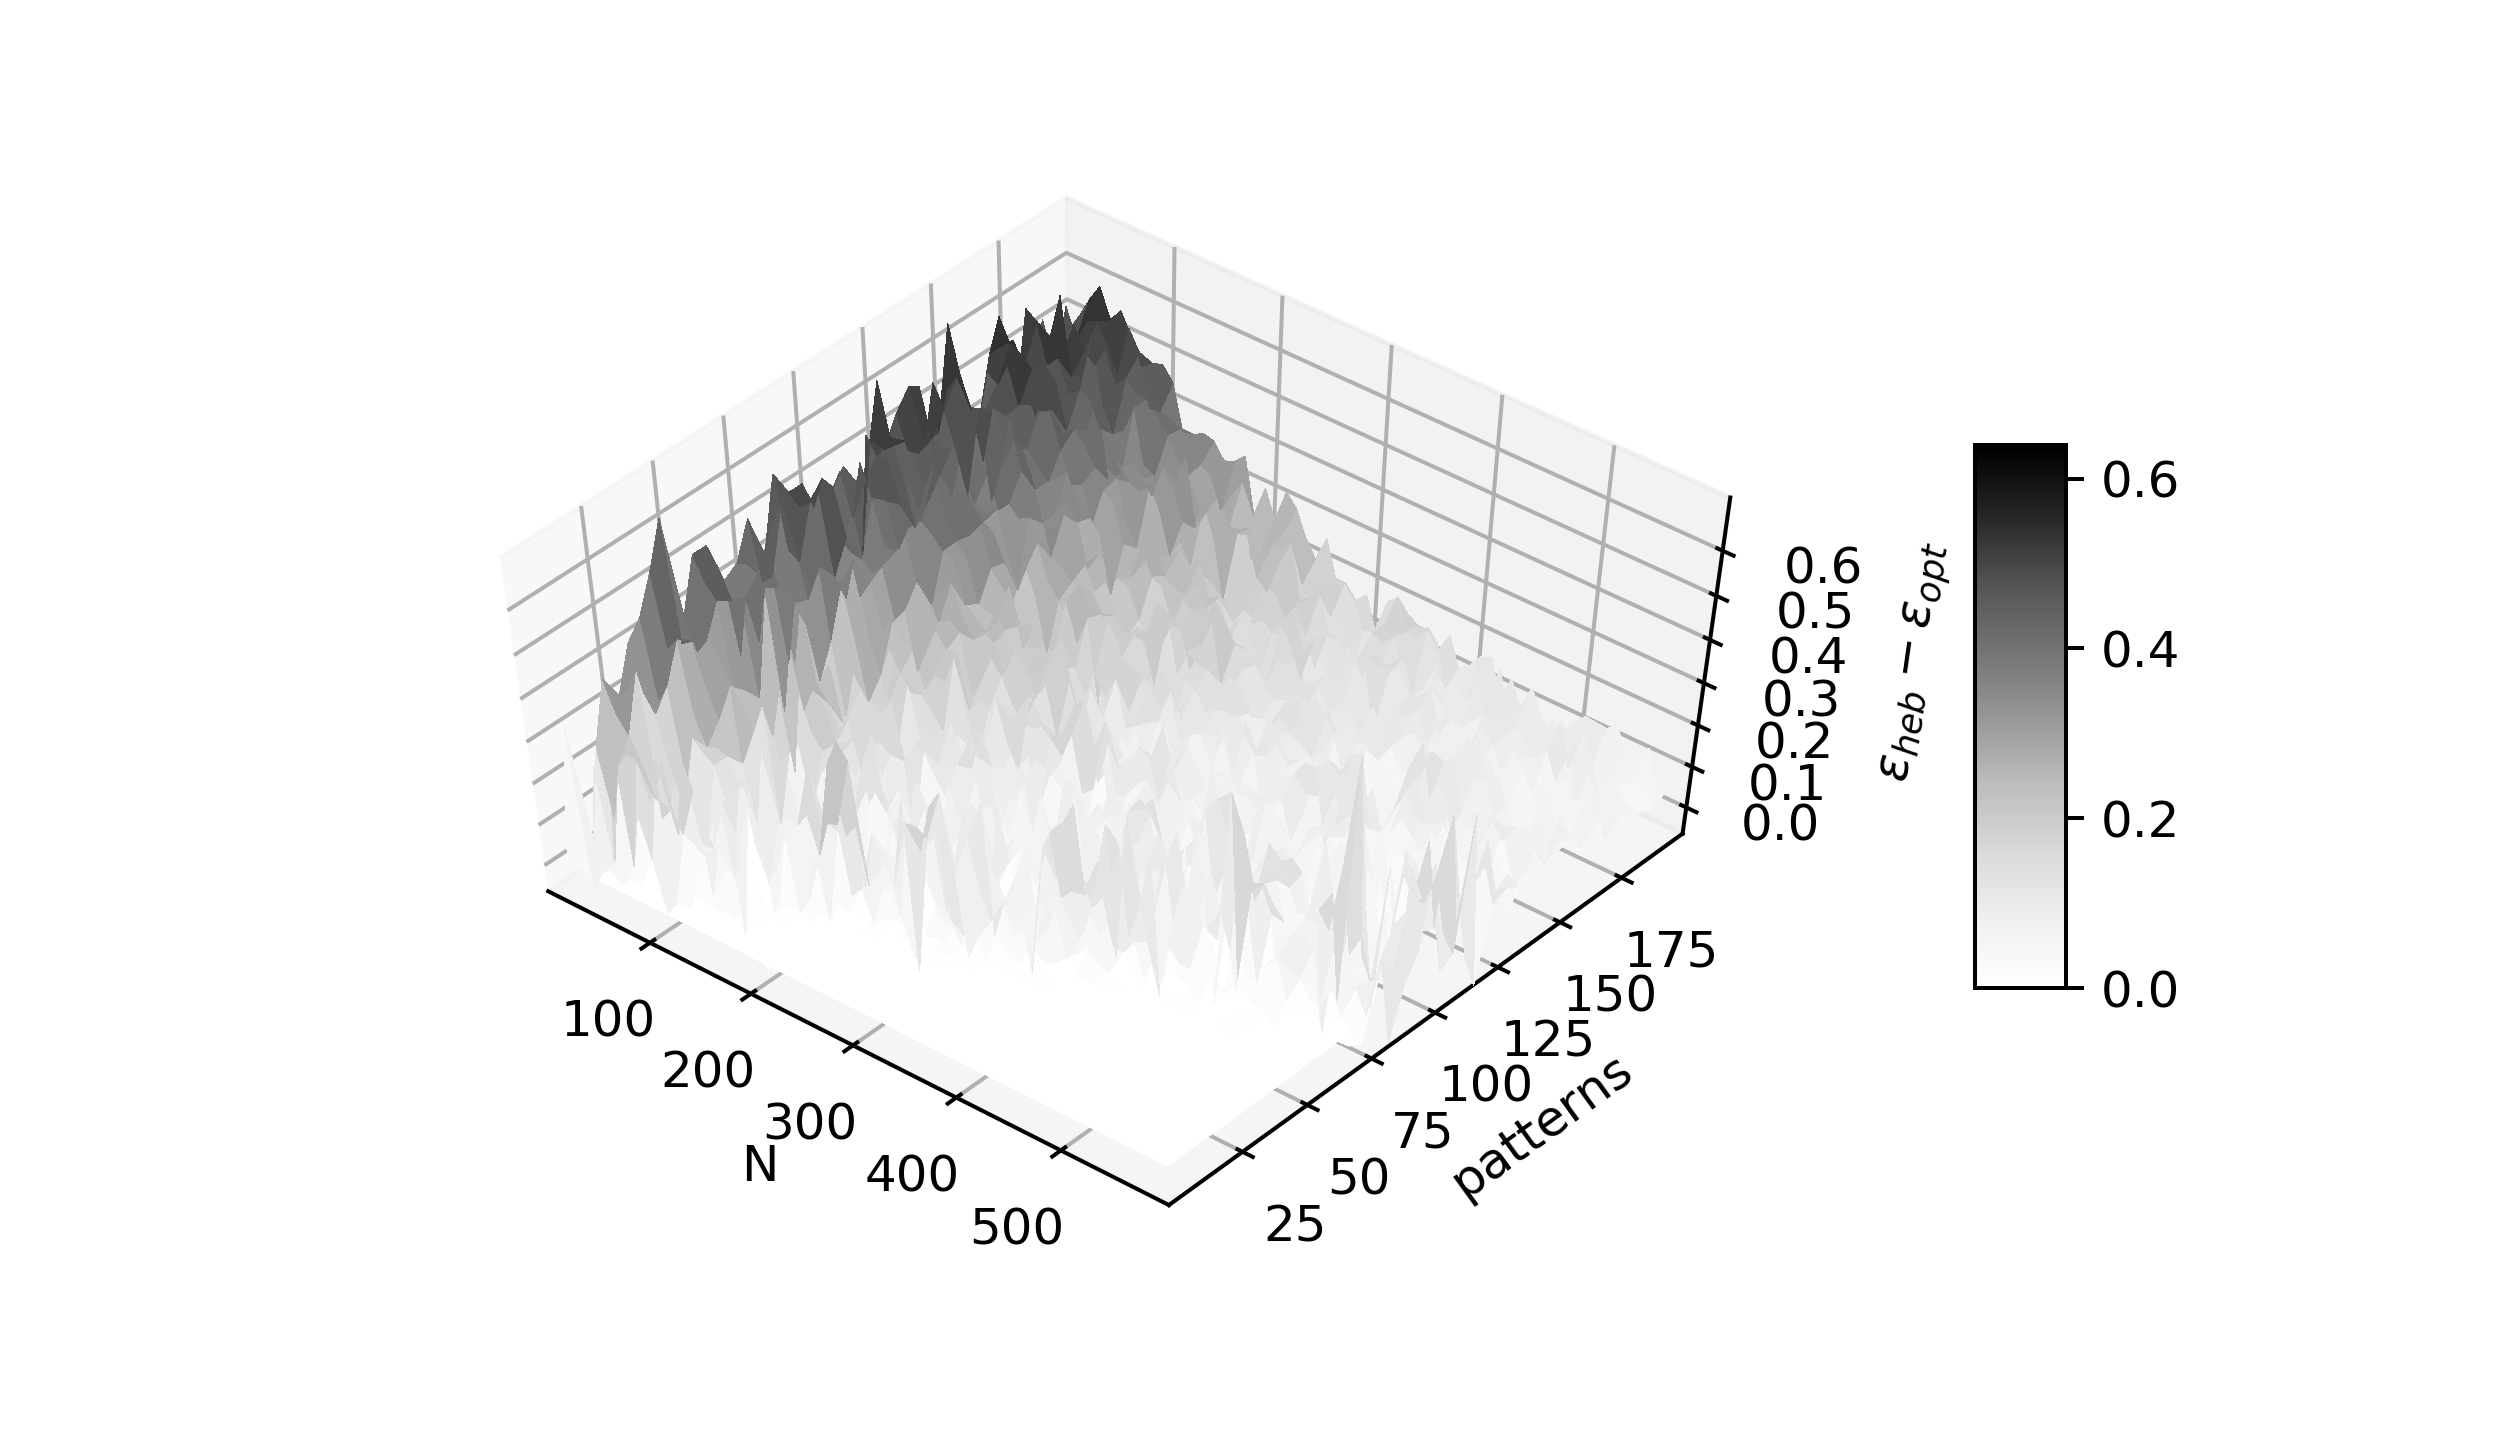
\includegraphics[width = 1.0\linewidth, trim={90 30 50 45}, clip=true]{scan_N_npat_hebopt.png}
		\subcaption{Difference in error between Hebbian weights and optimized weights across $(N, n_{opt})$ parameter space. All values are positive suggesting that the optimized weights always outperform the Hebbian weights.}
		\label{fig:hebopt}	
	\end{subfigure}%
	\hspace{0.001\linewidth}
	\begin{subfigure}[t]{0.45\linewidth}
		\centering
		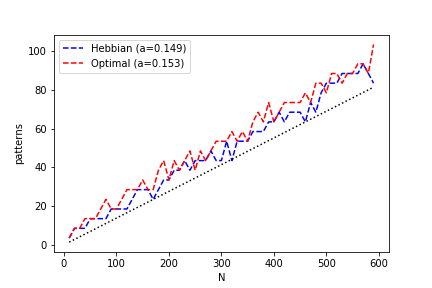
\includegraphics[width = 1.0\linewidth, trim={0 7 0 0}, clip=true]{compare_thresh.png}
		\subcaption{Capacity of Hebbian (blue) and optimized (red) networks as a function of N. Black dotted line corresponds to the Amit et al. model of a capacity of 0.138N.}
		\label{fig:heboptthresh}	
	\end{subfigure}%
\end{figure}

Of course this sort of network is only useful because the brain can make sense of the patterns it has stored; i.e. it can decode the information stored in a given pattern of states. Similarly, we can view learned patterns in our Hopfield network as a binary string of length N in which we can encode any information for which autoassociative recall might be desirable.

A simple example of this that we encounter every day is in text autocorrection and autocompletion. We can view the dictionary as a set of stored patterns, and our misspelled word as a faulty query. Any given misspelled word is likely to have only a few typos and we thus often query with more than 70\% of the training data, suggesting that this is a task we can use our Hopfield network to solve. Similarly, in an autocompletion process, we might give our network half a sentence and expect it to return the full sentence.

In order to achieve this, we first implement methods for converting an arbitrary lowercase string of length $n$ first to the corresponding 7-digit binary representation for each letter and then to a list of $-1$ and $+1$ of length $7n$. In this case we require the size of our network to be a multiple of 7, $N = 7i$ where i is an integer. We then add spaces as filling characters to make up for the difference in length between our query string and the capacity of the network since we must train the network with patterns of length $N$. We also implement a method to decode a given pattern into a string using the inverse methodology.

Given these functions, we can now train out network with a set of strings using the optimized strategy to learn weights since this outperforms Hebbian learning. As an example of autocorrection, we construct a net of size $N=84$ corresponding to a maximum if 12 characters. We then train it on the three strings ['hopfield', 'onomatopoeia', 'accommodate'].

Now when we try to write our report on hopfield networks, but accidentally think they were developed by John Ho\textbf{b}field, we get\\
\textit{network.query\_string('hobfield') $\rightarrow$ 'hopfield'}\\
Similarly, when we forget how to spell onomatopoeia, we get\\
\textit{network.query\_string('onomatopeia') $\rightarrow$ 'onomatopoeia'}\\

However, this implementation is strictly dependent on exact character matching in terms of location. Thus when we forget that 'accommodate' has two c's and two m's, all of the subsequent characters are mismatched and we fail to recover our original word\\
\textit{network.query\_string('acommodate') $\rightarrow$ 'iocoieodedia'}\\

Similarly, we can use a hopfield network for sentence autocompletion if we teach it a set of sentences. In the present case, we initialize a network with $N=235$ corresponding to 35 characters and learn weights for the following set of strings: ['i hope stephen gives me a good mark', 'i really like chocolate mousse', 'i really like strawberries with milk'].
We then query the network with a partial sentence:\\
\textit{network.query\_string('i hope stephen') $\rightarrow$ 'i hope stephen gives me a good mark'}\\

However, in the case of ambiguity, the network tends to fail and give a mixed result:\\
\textit{network.query\_string('i really like') $\rightarrow$ 'i really like sdkcgbete ewuwkdh ijmk'}\\

And as above, we are dependent on strict positional character matching:\\
\textit{network.query\_string('strawberries with milk') $\rightarrow$ 'i really like chocolate mousse'}\\
\textit{network.query\_string('\,\,\,\,\,\,\,\,\,\,\,\,\,\,\,\,\,\,\,\,\,\,\,\,\,\,\,\,\,\,\,\,\,\, strawberries with milk') $\rightarrow$ 'i really like strawberries with milk'}\\

Of course noone would actually use a Hopfiel network for  autocompletion and autocorrection in practice as there are many smarter algorithm in place that can also take into account contextual information and which have much higher capacities and superior recall. However, the above serves as an illustration that such networks are not limited to random patterns and visual representations, since this would be of little use to the brain. Instead they can be used for autoassociative recall of any information that can be encoded and decoded as binary strings.

\section*{Appendix}

\lstinputlisting[language=python]{if_neurons.jl}



\end{document}

\begin{table}[h]
\centering
\begin{tabular}{ |c|c|c|c|}
\hline
 & Sample size & Allele frequency \\
\hline
Selected population & 124 & 0.43 \\
\hline
Unselected population & 176 & 0.34 \\
\hline
\end{tabular}
\caption{Collected data}
\label{tab:data}
\end{table}